\documentclass{beamer}
%\usetheme{metropolis}
%\usepackage{cite}
\usepackage{amssymb}
\usepackage{graphicx}
\usepackage{url}
\usepackage{subcaption}
% Comment out the line below if using A4 paper size
%\usepackage[letterpaper]{geometry} % Uncomment both for slides...
%\usepackage{ltexpprt}
\usepackage{hyperref}
\usepackage{listings}
\usepackage{float}
\usepackage{wrapfig}
\usepackage{import}
\usepackage{booktabs}
\usepackage{siunitx}
\usepackage{algorithm}
\usepackage{algorithmic}
\usepackage{amsmath}
%\usepackage{footmisc}
\usepackage{multirow}

\newcommand{\email}[1]{\protect\href{mailto:#1}{#1}}

\title{\Large Tuning Spectral Element Preconditioners for Parallel Scalability on GPUs}

% Authors: full names plus addresses.
\author{Malachi Phillips\thanks{Department of Computer Science, University of Illinois at Urbana-Champaign
  (\email{malachi2@illinois.edu}).
  }
\and Stefan Kerkemeier\thanks{Mathematics and Computer Science, Argonne National Laboratory
  (\email{kerkemeier@anl.gov}).
  }
\and Paul Fischer$^{*\dagger}$\thanks{Department of Mechanical Science and Engineering,
University of Illinois at Urbana-Champaign
(\email{fischerp@illinois.edu}).
  }
}

\usepackage[export]{adjustbox}
\usepackage[style=authortitle,backend=bibtex]{biblatex}
\addbibresource{paper.bib}
\usepackage{enumitem}
\setlistdepth{9}

\setlist[itemize,1]{label=$\bullet$}
\setlist[itemize,2]{label=$\bullet$}
\setlist[itemize,3]{label=$\bullet$}
\setlist[itemize,4]{label=$\bullet$}
\setlist[itemize,5]{label=$\bullet$}
\setlist[itemize,6]{label=$\bullet$}
\setlist[itemize,7]{label=$\bullet$}
\setlist[itemize,8]{label=$\bullet$}
\setlist[itemize,9]{label=$\bullet$}

\renewlist{itemize}{itemize}{9}
%\usepackage{enumitem}
%\usepackage{natbib}

% re-state institute in Beamer form
\author{
Malachi Phillips\inst{1}
  \and
Stefan Kerkemeier\inst{2}
  \and
Paul Fischer\inst{1,2,3}
}

\institute[shortinst]{
  \inst{1} Department of Computer Science, University of Illinois at Urbana-Champaign
  \and
  \inst{2} Mathematics and Computer Science, Argonne National Laboratory, Lemont, IL 60439
  \and
  \inst{3} Department of Mechanical Science and Engineering, University of Illinois at Urbana-Champaign
}

\usepackage{float} %figure inside minipage

% useful defines
\def\dO{\partial \Omega}
\def\Oh{{\hat \Omega}}
\def\uu{{\underline u}}
\def\ur{{\underline r}}
\def\us{{\underline s}}
\def\uf{{\underline f}}
\def\tlam {{\tilde \lambda}}

\begin{document}
\date{}
%\maketitle

\begin{frame}{Poisson}
  \begin{itemize}
    \item Poisson solve encompasses the majority of the solution time.
    \item Spectral element (SE): $E$ elements with polynomial degree $p$, $n\approx E p^3$ unknowns and $\mathcal O(Ep^6)$ nonzeros.
    \begin{itemize}
      \item Matrix-free is a must: exploit tensor-product-sum factorization, $\mathcal O(Ep^4)$ cost to apply matrix-vector product \footcite{deville_high-order_2002}.
      \item Poor conditioning of system: $\kappa(A)\sim\mathcal O(h^{-p})$ requires preconditioning.
    \end{itemize}
  \end{itemize}
\end{frame}

%--------------------------------------------------------------------------
% Structure of talk
%--------------------------------------------------------------------------
%\input{slides/structure} % Not needed for a 15 minute talk...

%--------------------------------------------------------------------------
% Overview of preconditioning techniques
%--------------------------------------------------------------------------
\begin{frame}{Solvers}
  \begin{itemize}
    \item Solution projection for initial guess generation \footcite{fischer_projection_1998}
    \item Krylov subspace projection methods:
    \begin{itemize}
      \item flexible PCG
      \item PGMRES
    \end{itemize}
    \item Preconditioners:
    \begin{itemize}
      \item Low-order operator preconditioning (SEMFEM)
      \item Geometric $p$-Multigrid (pMG), requiring a smoother:
      \begin{itemize}
        \item Additive Schwarz (ASM) and restrictive additive Schwarz (RAS)
        \item Chebyshev polynomial smoothing
        \begin{itemize}
          \item Jacobi
          \item ASM, RAS
        \end{itemize}
      \end{itemize}
    \end{itemize}
  \end{itemize}
\end{frame}

%--------------------------------------------------------------------------
% SEMFEM Preconditioner
%--------------------------------------------------------------------------
\begin{frame}{SEMFEM}
  \begin{itemize}
    \item Precondition high-order system with low-order discretizations with coinciding nodes
    \item Orszag \footcite{parter_spectral_1979} demonstrated $\kappa(\mathbf M^{-1} \mathbf A) \sim \pi^2/4$ scaling for second-order Dirichlet problems.
    \item Bello-Maldonado and Fischer \footcite{bello-maldonado_scalable_2019} proposed using one-per-vertex scheme.
    \begin{itemize}
      \item{
        Same, but solve with AmgX \footcite{naumov_amgx_2015}
        single pass V-cycle, damped Jacobi relaxation ($\omega = 0.9$).
        }
    \end{itemize}
  \end{itemize}
  \vspace{-0.35cm}
  \begin{figure}
    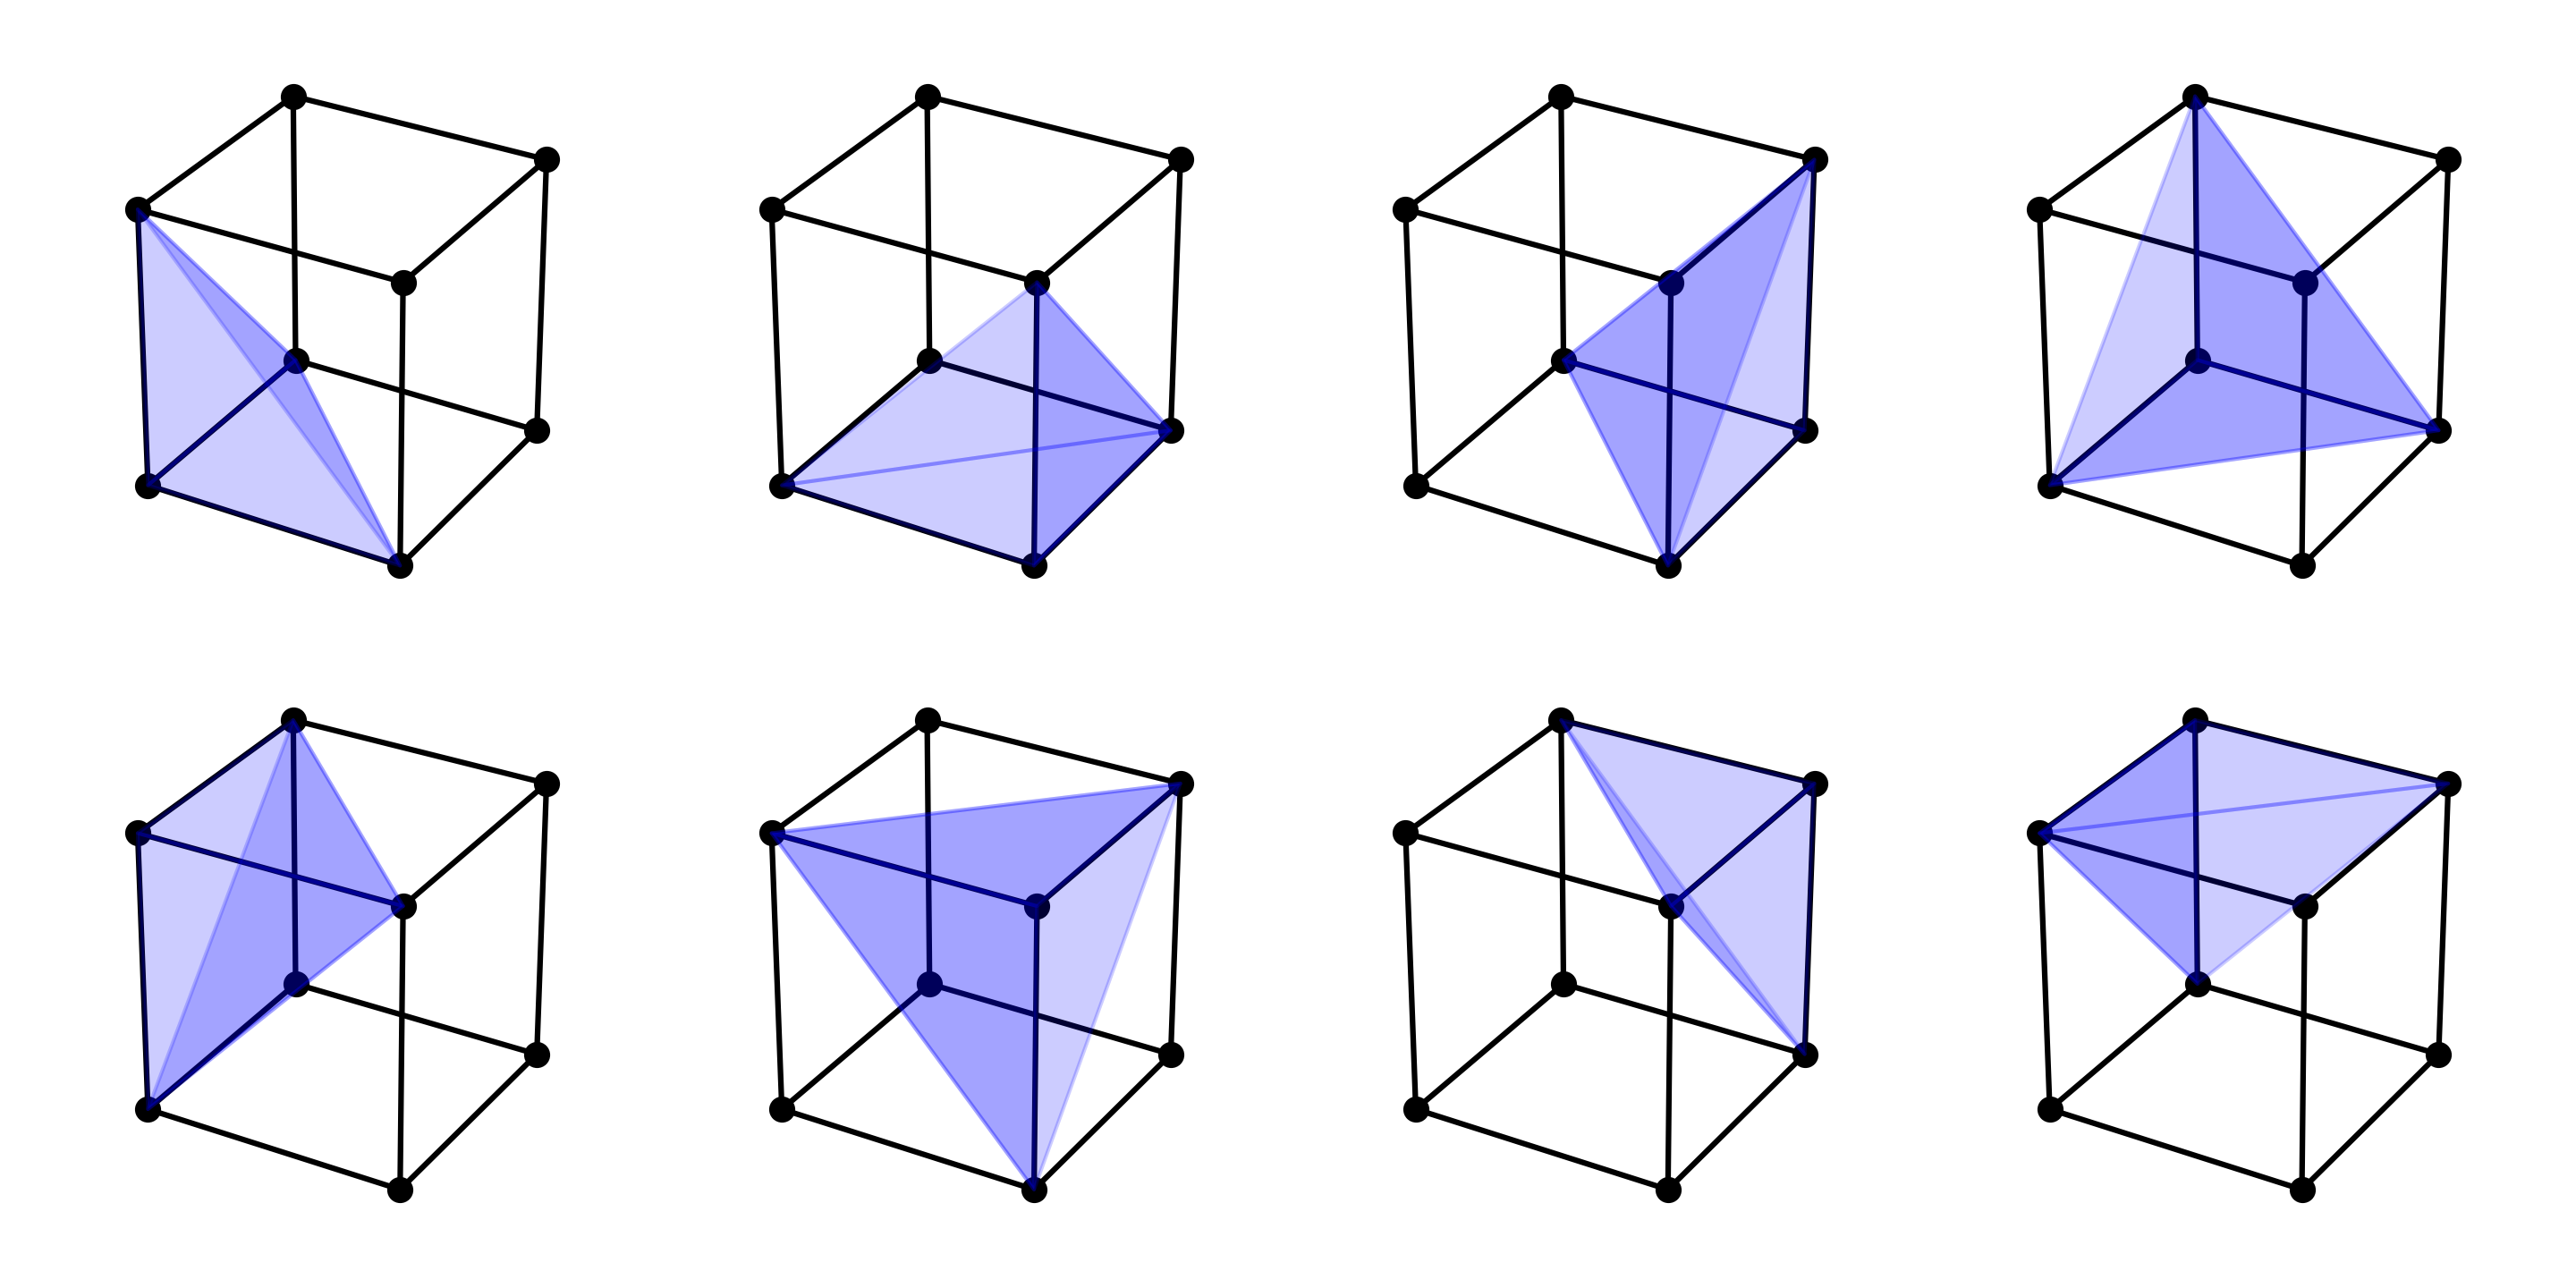
\includegraphics[width=0.5\textwidth]{../figs/one-tet-per-vertex.png}
    %\vspace{-0.35cm}
    %\caption{\label{fig:one-tet-per-vertex}
    %  \small
    %  Demonstration of one-per-vertex scheme.
    %}
  \end{figure}
\end{frame}

%--------------------------------------------------------------------------
% Multigrid Preconditioner and Smoothers
%--------------------------------------------------------------------------
%\begin{frame}{Multigrid}
  \begin{columns}
    \begin{column}{0.6\textwidth}
      \begin{algorithm}[H]\small
   \caption{Multigrid V-cycle}
   \label{alg:V-cycle}
   \begin{algorithmic}
    \STATE{$\mathbf x = \mathbf x + \mathbf M^{-1} (\mathbf b - \mathbf A\mathbf x)$ // smooth}
    \STATE{$\mathbf r = \mathbf b - \mathbf A \mathbf x$ // re-evaluate residual}
    \STATE{$\mathbf r_C = \mathbf P^T \mathbf r$ // coarsen }
    \STATE{$\mathbf e_C = \mathbf A_C^{-1} \mathbf r_C$ // solve/re-apply V-cycle }
    \STATE{$\mathbf e = \mathbf P \mathbf e_C$ // prolongate }
    \STATE{$\mathbf x = \mathbf x + \mathbf e$ // update solution }
    \STATE{$\mathbf x = \mathbf x + \mathbf M^{-1}(\mathbf b - A\mathbf x)$ // post smoothing }
   \end{algorithmic}
\end{algorithm}

      \vspace{-0.5cm}
      Smoother choices:
      \begin{itemize}
        \item Damped Jacobi
        \item Schwarz
        \item Chebyshev Jacobi smoothing
        \item \em{Chebyshev Schwarz smoothing}
      \end{itemize}
    \end{column}
    \begin{column}{0.4\textwidth}
      \begin{figure}
        %\begin{flushright}
        {\setlength{\unitlength}{\textwidth}
        \begin{picture}(1, 1.75)
          \put(0,0){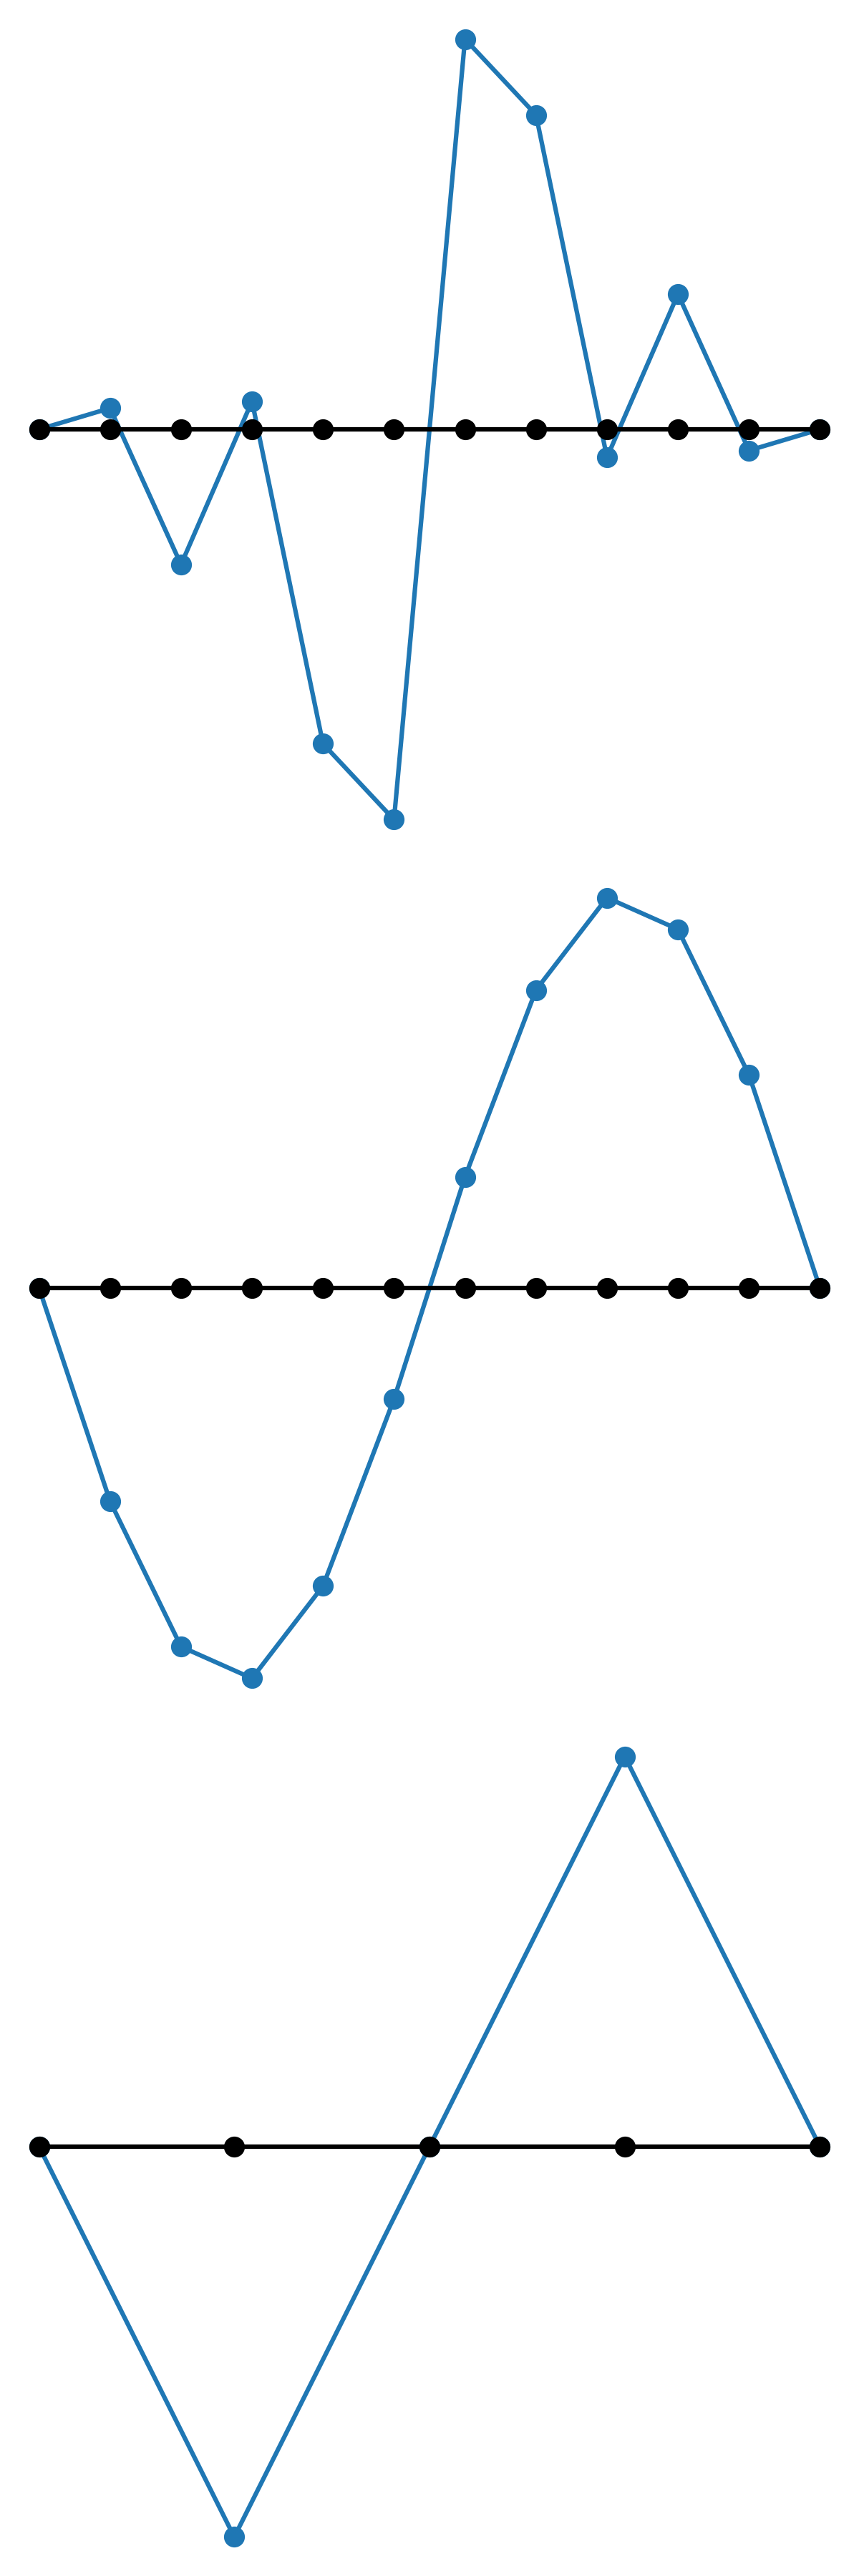
\includegraphics[height=0.8\textheight]{../figs/multigrid.png}}
          %\qbezier(0.2,1)(0.0,0.8)(0.2,0.6)
          \put(0.55, 1.2){\vector(0,-1){0.2}}
          \put(0.55, 0.6){\vector(0,-1){0.2}}
          \put(0.6, 1.1){\large Smooth}
          \put(0.6, 0.5){\large Coarsen}
        \end{picture}
        }
        %\end{flushright}
        %\vspace{-0.8cm}
        %\caption{\label{fig:mg-demo}
        %  \small
        %  Multigrid
        %}
      \end{figure}
    \end{column}
  \end{columns}
\end{frame}

%--------------------------------------------------------------------------
% Schwarz Smoothing Algorithm
%--------------------------------------------------------------------------
\begin{frame}{ASM, RAS Smoothers}
  \begin{figure} \centering
  {\setlength{\unitlength}{1\textwidth}
    \begin{picture}(1,0.35)
       \put(0.0,0.0){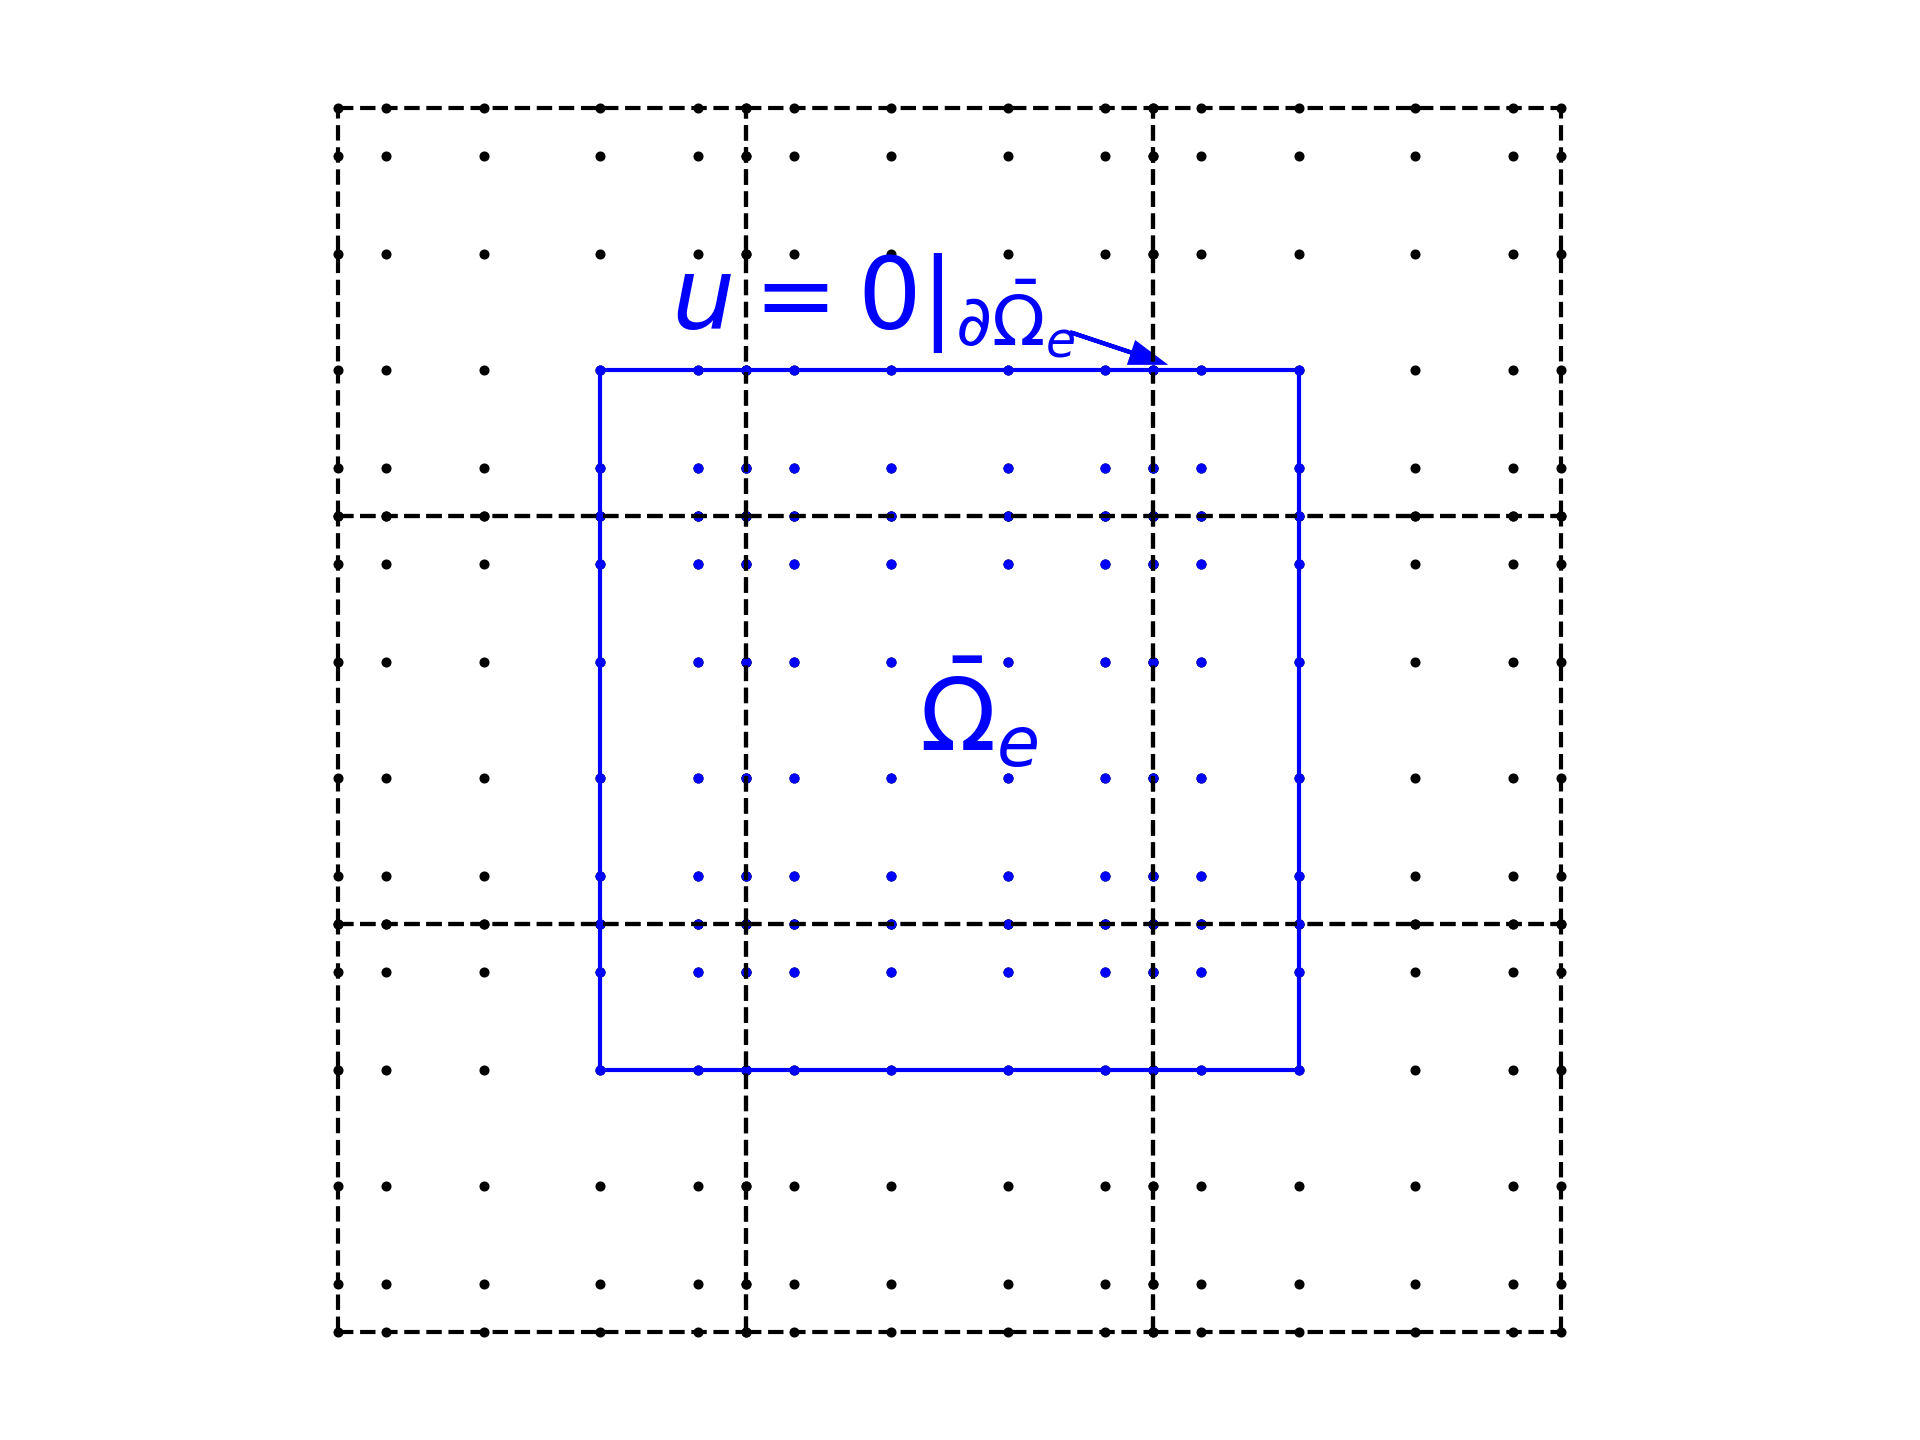
\includegraphics[width=0.5\textwidth]{../figs/overlapping-schwarz-diagram-p=5.png}}
       \put(0.5,0.0){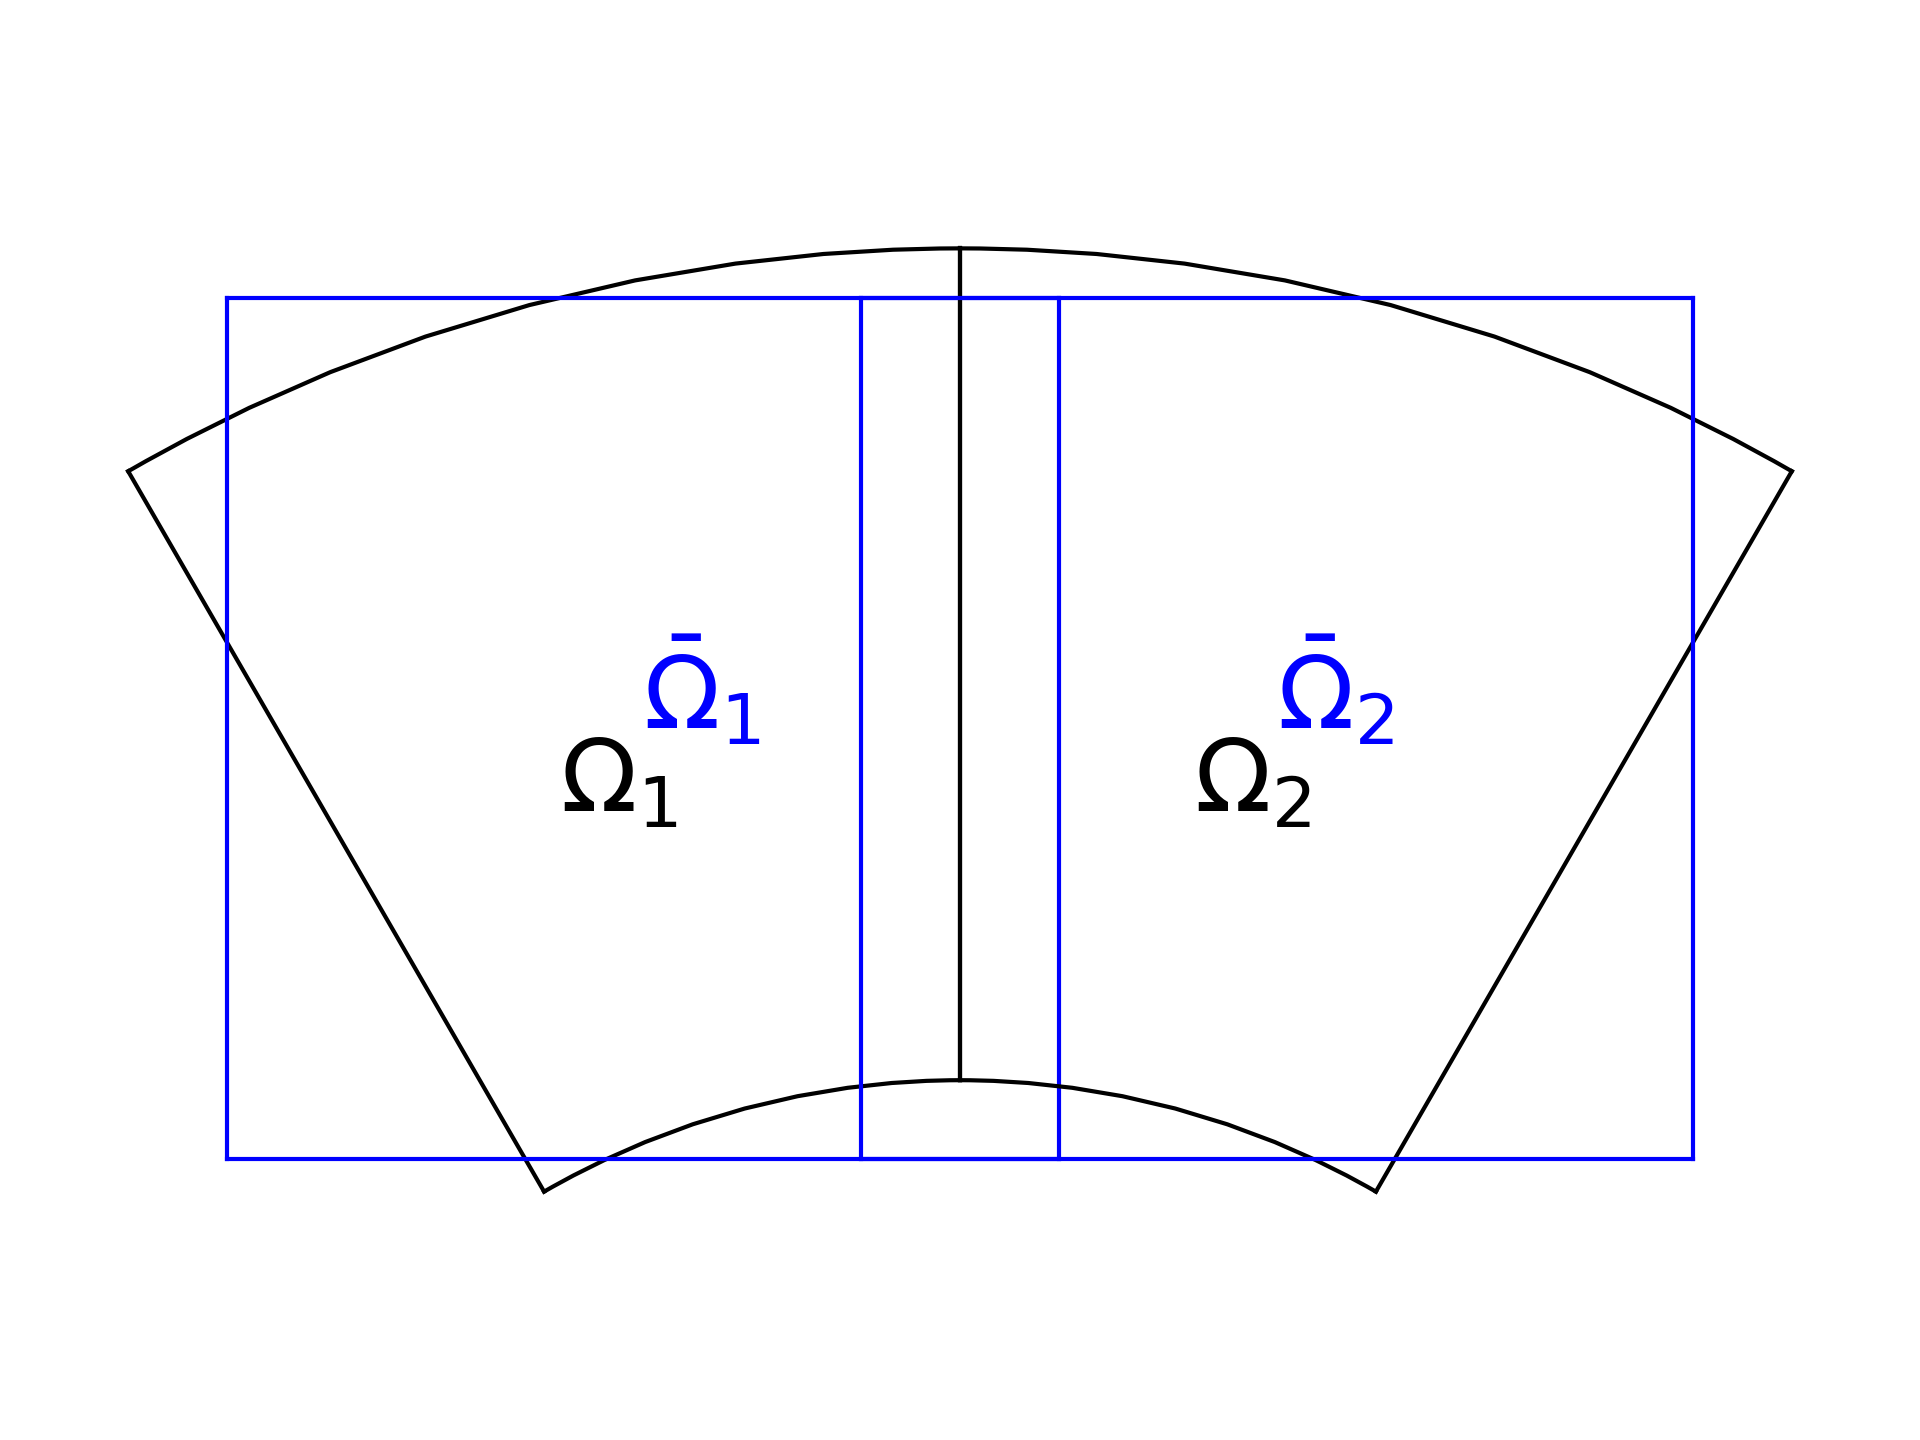
\includegraphics[width=0.5\textwidth]{../figs/schwarz-approximation.png}}
  
       \put(0.0,0.05){\large (a)}
       \put(0.45,0.05){\large (b)}
    \end{picture}
  }
  %\vspace{-0.4cm}
  %\caption{\label{fig:schwarz} Schwarz}
  \end{figure}
  \vspace{-0.65cm}
  \begin{itemize}
    \item $\mathbf M^{-1} := \sum_{e=1}^E \mathbf W_e \mathbf R_e^T \mathbf {\bar A}_e^{-1} \mathbf R_e$, subdomain (a) \footcite{lottes_hybrid_2005,loisel_hybrid_2008}.
    \item How to form $\mathbf {\bar A}_e^{-1}$?
    \begin{itemize}
      \item Galerkin: $\mathbf {\bar A}_e = \mathbf R_e \mathbf A \mathbf R_e^T$, ruins $\mathcal O(p^3)$ storage, $\mathcal O(p^4)$ work per element.
      \item Box-like approximation (b): recover $\mathcal O(p^3)$ storage, $\mathcal O(p^4)$ work per element using fast diagonalization method (FDM).
    \end{itemize}
  \end{itemize}
\end{frame}

%\begin{frame}{FDM}
%  \begin{itemize}
%    \item 3D Poisson-in-a-box:
%      \begin{equation*}\label{eq:tensor-prod-poisson}
%      \mathbf {\bar A} = \mathbf B_z \otimes \mathbf B_y \otimes \mathbf A_x
%               +\mathbf B_z \otimes \mathbf A_y \otimes \mathbf B_x
%               +\mathbf A_z \otimes \mathbf B_y \otimes \mathbf B_x,
%      \end{equation*}
%    \item Directly invert with FDM with $\mathcal O(p^3)$ storage, $\mathcal O(p^4)$ work:
%      \begin{equation*}\label{eq:inverse-tensor-prod-poisson}
%      {\bar A}^{-1} = 
%      (S_z\otimes S_y\otimes S_x) D^{-1} (S_z^T \otimes S_y^T \otimes S_x^T),
%      \end{equation*}
%      where
%      \begin{equation*}
%      D=I\otimes I\otimes \Lambda_x+I\otimes \Lambda_y \otimes I+\Lambda_z \otimes I \otimes I
%      \end{equation*}
%      and each $\mathbf S_*$, $\mathbf \Lambda_*$ are from the generalized eigenvalue problem:
%      \begin{equation*}\label{eq:generalized-eig}
%      \mathbf A_* \mathbf{s}_i = \lambda_i \mathbf B_* \mathbf{s}_i
%      \end{equation*}
%      where $\mathbf B_*$, $\mathbf A_*$ are 1D mass-stiffness matrices.
%  \end{itemize}
%
%\end{frame}

%--------------------------------------------------------------------------
% Chebyshev Smoothing Algorithm
%--------------------------------------------------------------------------
\begin{frame}{Chebyshev Smoothing}
\begin{itemize}
  \item Construct Chebyshev polynomial of $\mathbf {SA}$ minimum in interval $[\lambda_{min}, \lambda_{max}]$.
  \item Max eigenvalue estimate $\tilde{\lambda}$ obtained with 10 Arnoldi iterations,
        $(\lambda_{max}, \lambda_{min}) = (1.1,0.1)\tilde{\lambda}$.
  \item $\mathbf S = \operatorname{invDiag}(A)$ \footcite{adams_parallel_2003, Kronbichler2019}, or, more recently, a Schwarz smoother \footcite{phillips-tuning-2022}
  \begin{itemize}
    \item Chebyshev-acceleration \emph{robustifies} point wise smoother (Jacobi)
    \item Similarly, Chebyshev-acceleration applied to Schwarz smoothers improves multigrid convergence
  \end{itemize}
\end{itemize}
\end{frame}

%--------------------------------------------------------------------------
% Test cases
%--------------------------------------------------------------------------
\begin{frame}{Navier-Stokes}
  \begin{columns}
    \begin{column}{0.45\textwidth}
      \begin{figure}
        \begin{flushleft}
          {\setlength{\unitlength}{\textwidth}
            \begin{picture}(1,1.5)(0,0)
              \put(0.0,0.75){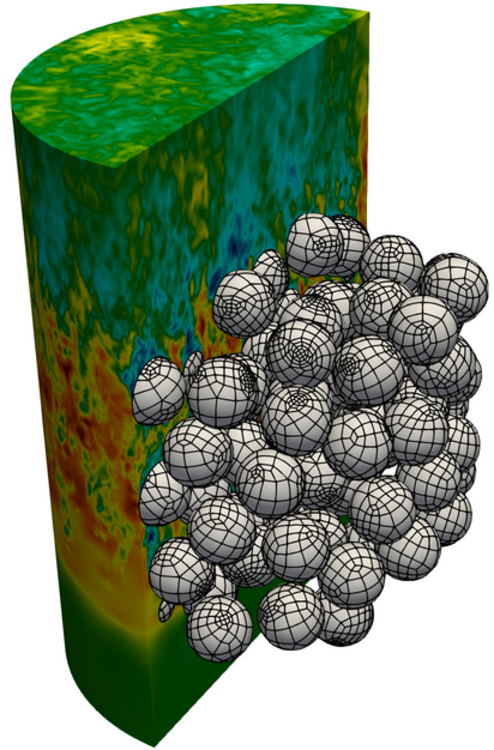
\includegraphics[width=0.45\textwidth, left]{../figs/pb146.png}}
              \put(0.5,0.75){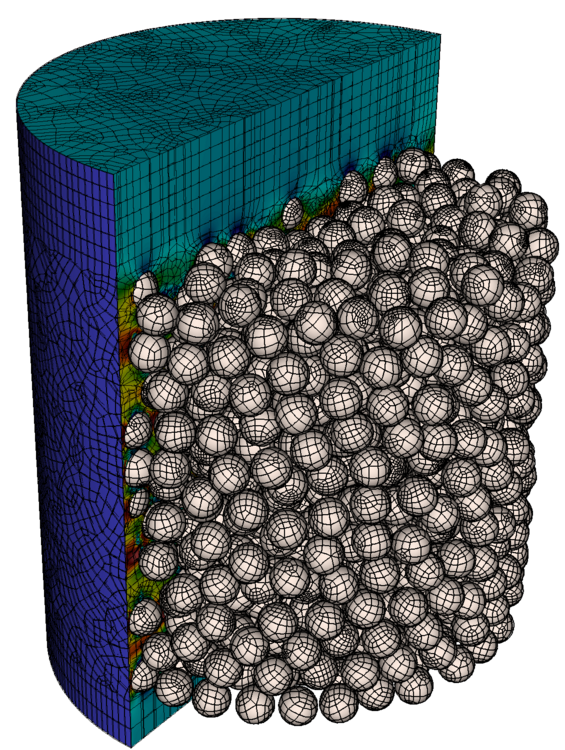
\includegraphics[width=0.5\textwidth, left]{../figs/pb1568.png}}
              \put(0.0,0.40){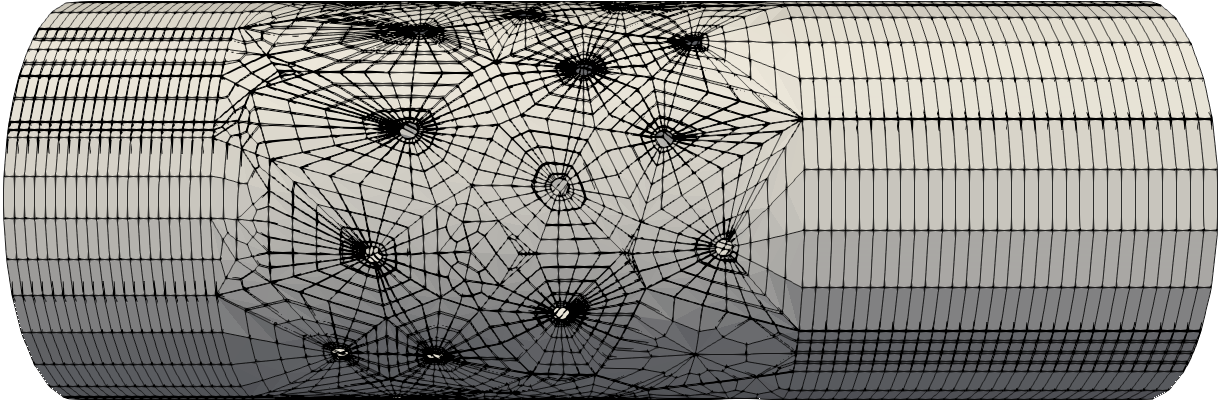
\includegraphics[width=0.9\textwidth, right]{../figs/peb67-side-profile.png}}
              \put(0.0,0.00){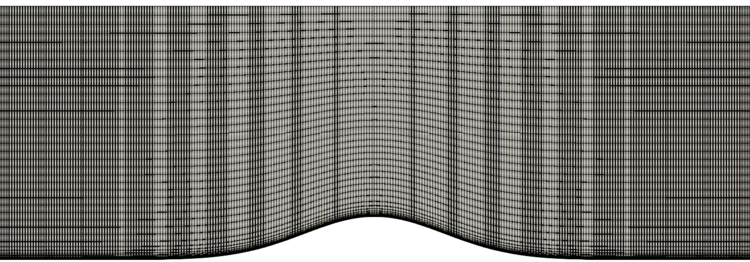
\includegraphics[width=0.9\textwidth, right]{../figs/BoeingSpeedBump.png}}

              \put(-0.05,0.80){\large (a)}
              \put(0.40,0.80){\large (b)}
              \put(-0.05,0.45){\large (c)}
              \put(-0.05,0.05){\large (d)}
  
            \end{picture}}
        \end{flushleft}
      \end{figure}
    \end{column}
    \begin{column}{0.55\textwidth}
      \begin{table}\tiny
\begin{tabular}{||c| c c c ||}
  \hline
  Case Name & $E$ & $p$ & $n$\\
  \hline\hline
  146 pebble  (a) & 62K & 7 & 21M\\
  1568 pebble (b) & 524K & 7 & 180M\\
  67 pebble   (c) & 122K & 7 & 42M\\
  Speed bump  (d) & 885K & 9 & 645M\\
\hline
  & CFL & $\Delta t$ & $T_{restart}$\\
  \hline \rule{0pt}{2.5ex} 
  %(a) \footcite{lan_all-hex_2021} & 4 & $2\times 10^{-3}$ & 10\\
  %(b) \footcite{lan_all-hex_2021} & 4 & $5\times 10^{-4}$ & 20\\
  %(c) \footcite{yuan2020spectral} & 4 & $5\times 10^{-5}$ & 10.6\\
  %(d) \footcite{shur_direct_2021} & 0.8 & $2\times 10^{-3}$ & 5.6\\
  (a) & 4 & $2\times 10^{-3}$ & 10\\
  (b) & 4 & $5\times 10^{-4}$ & 20\\
  (c) & 4 & $5\times 10^{-5}$ & 10.6\\
  (d) & 0.8 & $2\times 10^{-3}$ & 5.6\\
  \hline
  & $Re$ & Tol & Steps \\
  \hline \rule{0pt}{2.5ex} 
  (a) & $5000$ & $10^{-4}$ & 2000\\
  (b) & $5000$ & $10^{-4}$ & 2000\\
  (c) & $1460$ & $10^{-4}$ & 2000\\
  (d) & $10^6$ & $10^{-5}$ & 2000\\
  \hline
\end{tabular}
\captionsetup{labelformat=empty}
\caption{
  \small
  %Problem discretization, timestepping parameters.
  %Pebble cases use a two stage subcycling scheme.
  %All cases use a 2nd-order timestepper with 10 prior solution vectors
  %to generate the initial guess%. \cite{fischer_projection_1998}.
  \label{table:problem-sizes}
}
\end{table}
    \end{column}
    \end{columns}
\end{frame}

%--------------------------------------------------------------------------
% Results
%--------------------------------------------------------------------------
\begin{frame}{Results}
  \begin{itemize}
    \item All results on Summit (42 IBM Power9 CPUs, 6 NVIDIA V100 GPUs per node).
    \item Each of the $P$ ranks are assigned one GPU, 6 GPUs per node (unless $P<6$).
    \item At coarsest level, solve using one BoomerAMG V-cycles \footcite{henson_boomeramg_2002}
    \item pMG (7,3,1), Cheby-ASM(2) denotes pMG preconditioning with a 2nd-order Chebyshev-accelerated ASM smoother with %three
    $p=7$, $p=3$, and $p=1$ as multigrid levels.
  \end{itemize}
\end{frame}
\begin{frame}
  %\begin{figure}
  %  \centering
  %  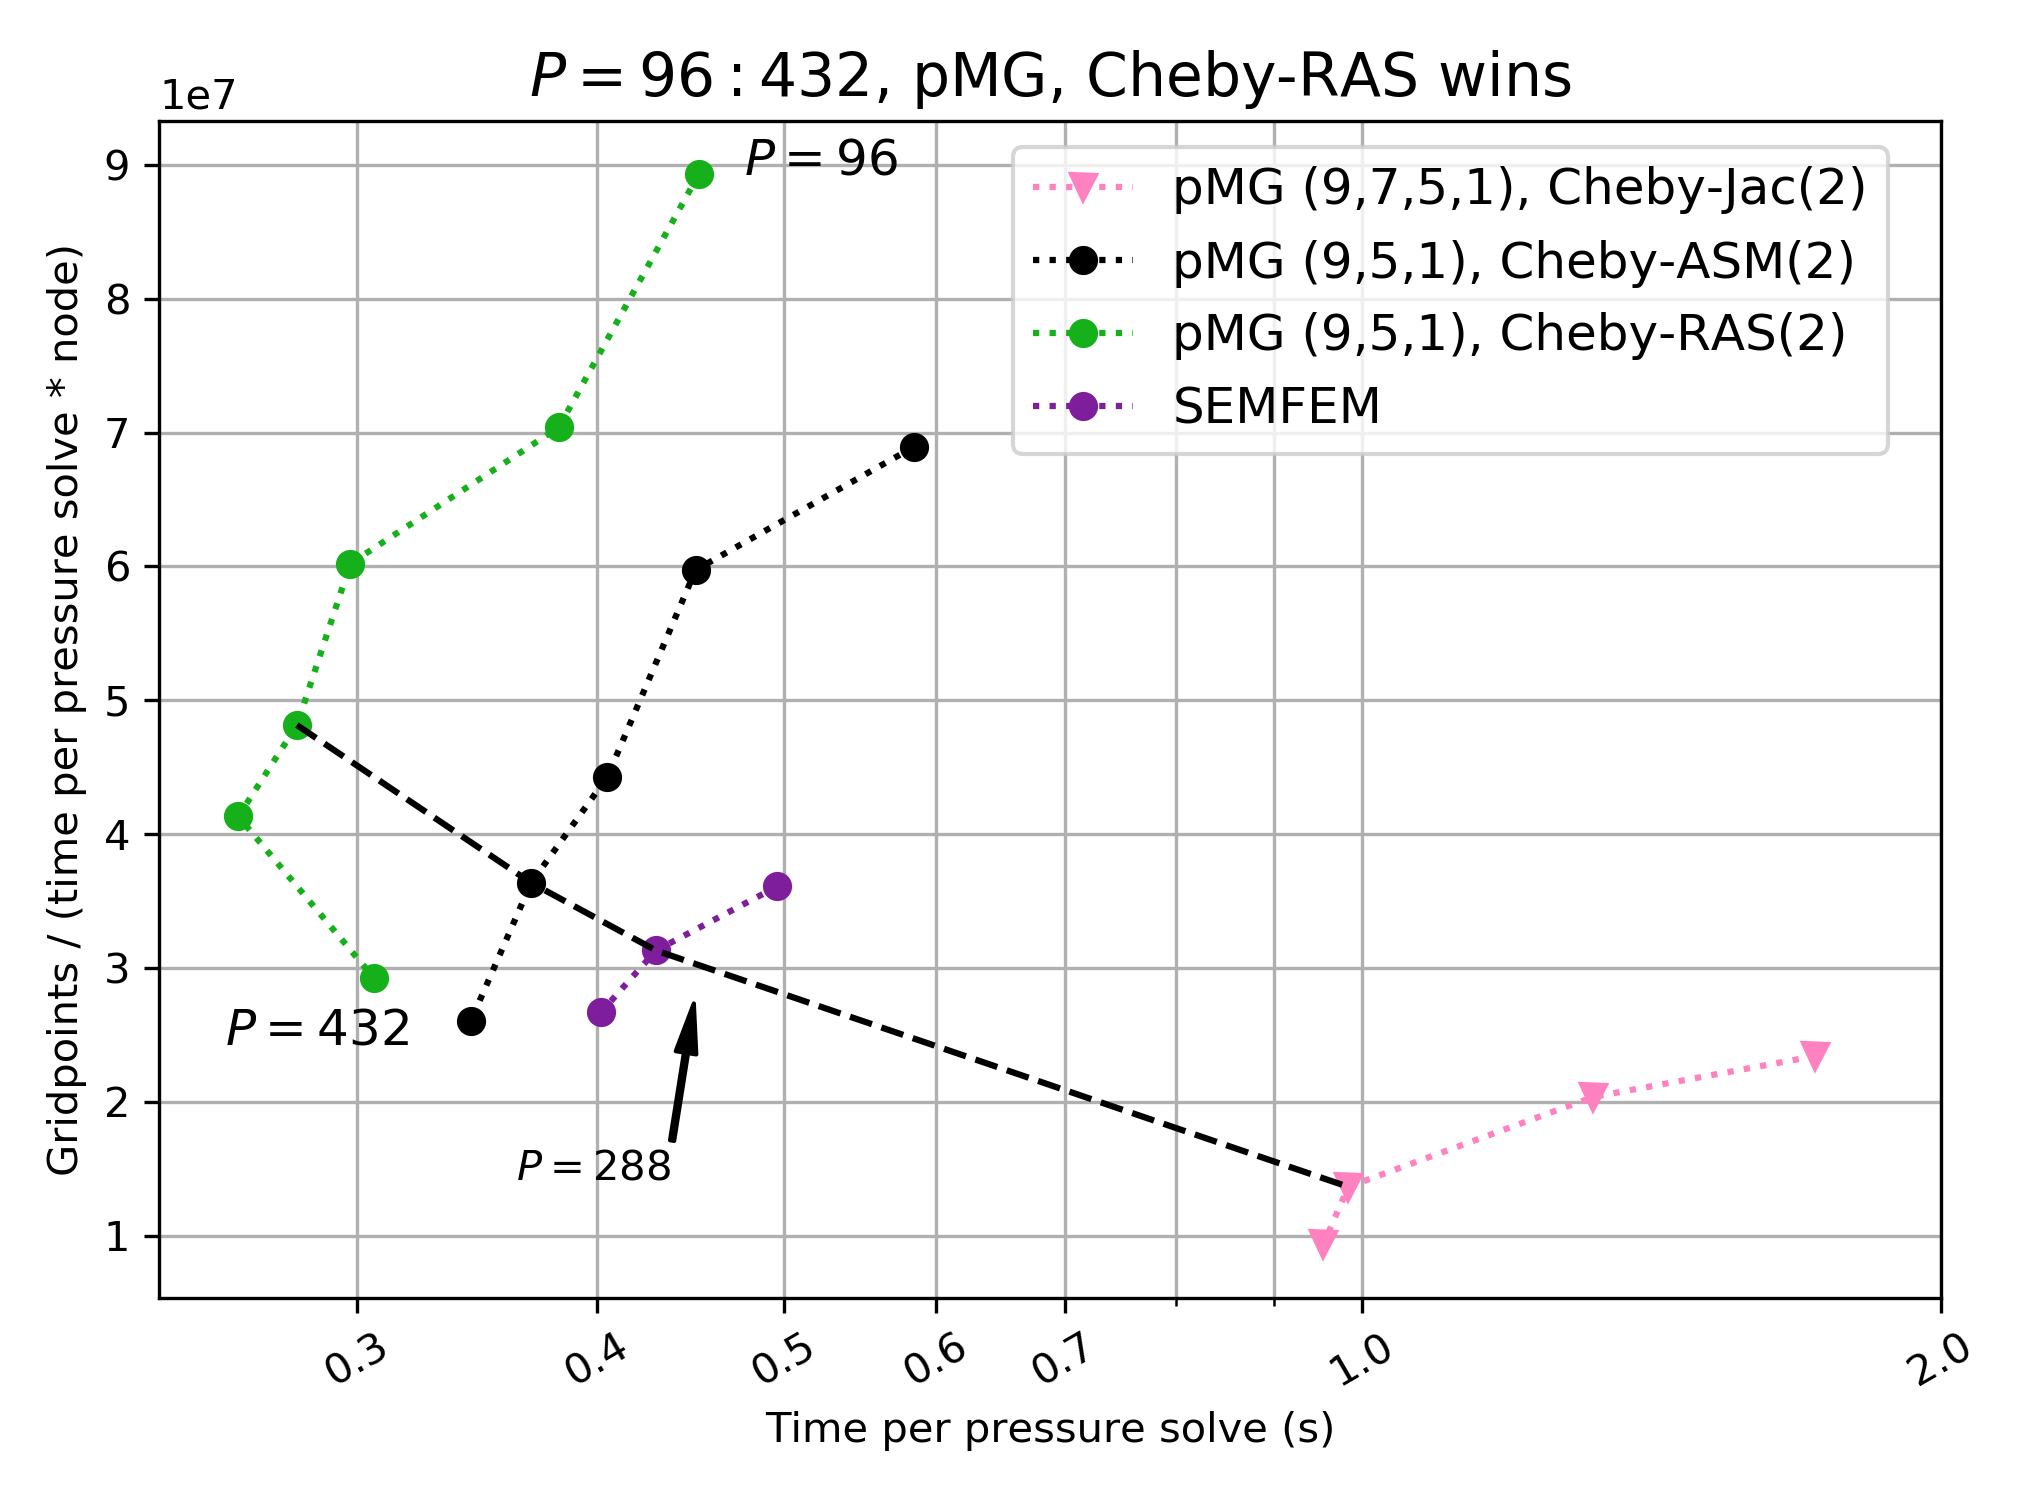
\includegraphics[width=\textwidth]{../figs/bsb-scaling.png}
  
  %  \vspace{-0.35cm}
  %  \captionsetup{labelformat=empty}
  %  \caption{
  %    \small
  %    Strong scaling results on Summit for the Boeing speed bump problem.
  %  }
  %  \label{fig:scaling-study-bsb}
  
  %\end{figure}
  \begin{figure}
    {\setlength{\unitlength}{\textwidth}
      \begin{picture}(1,0.75)(0,0)
        \put(0.0,0.0){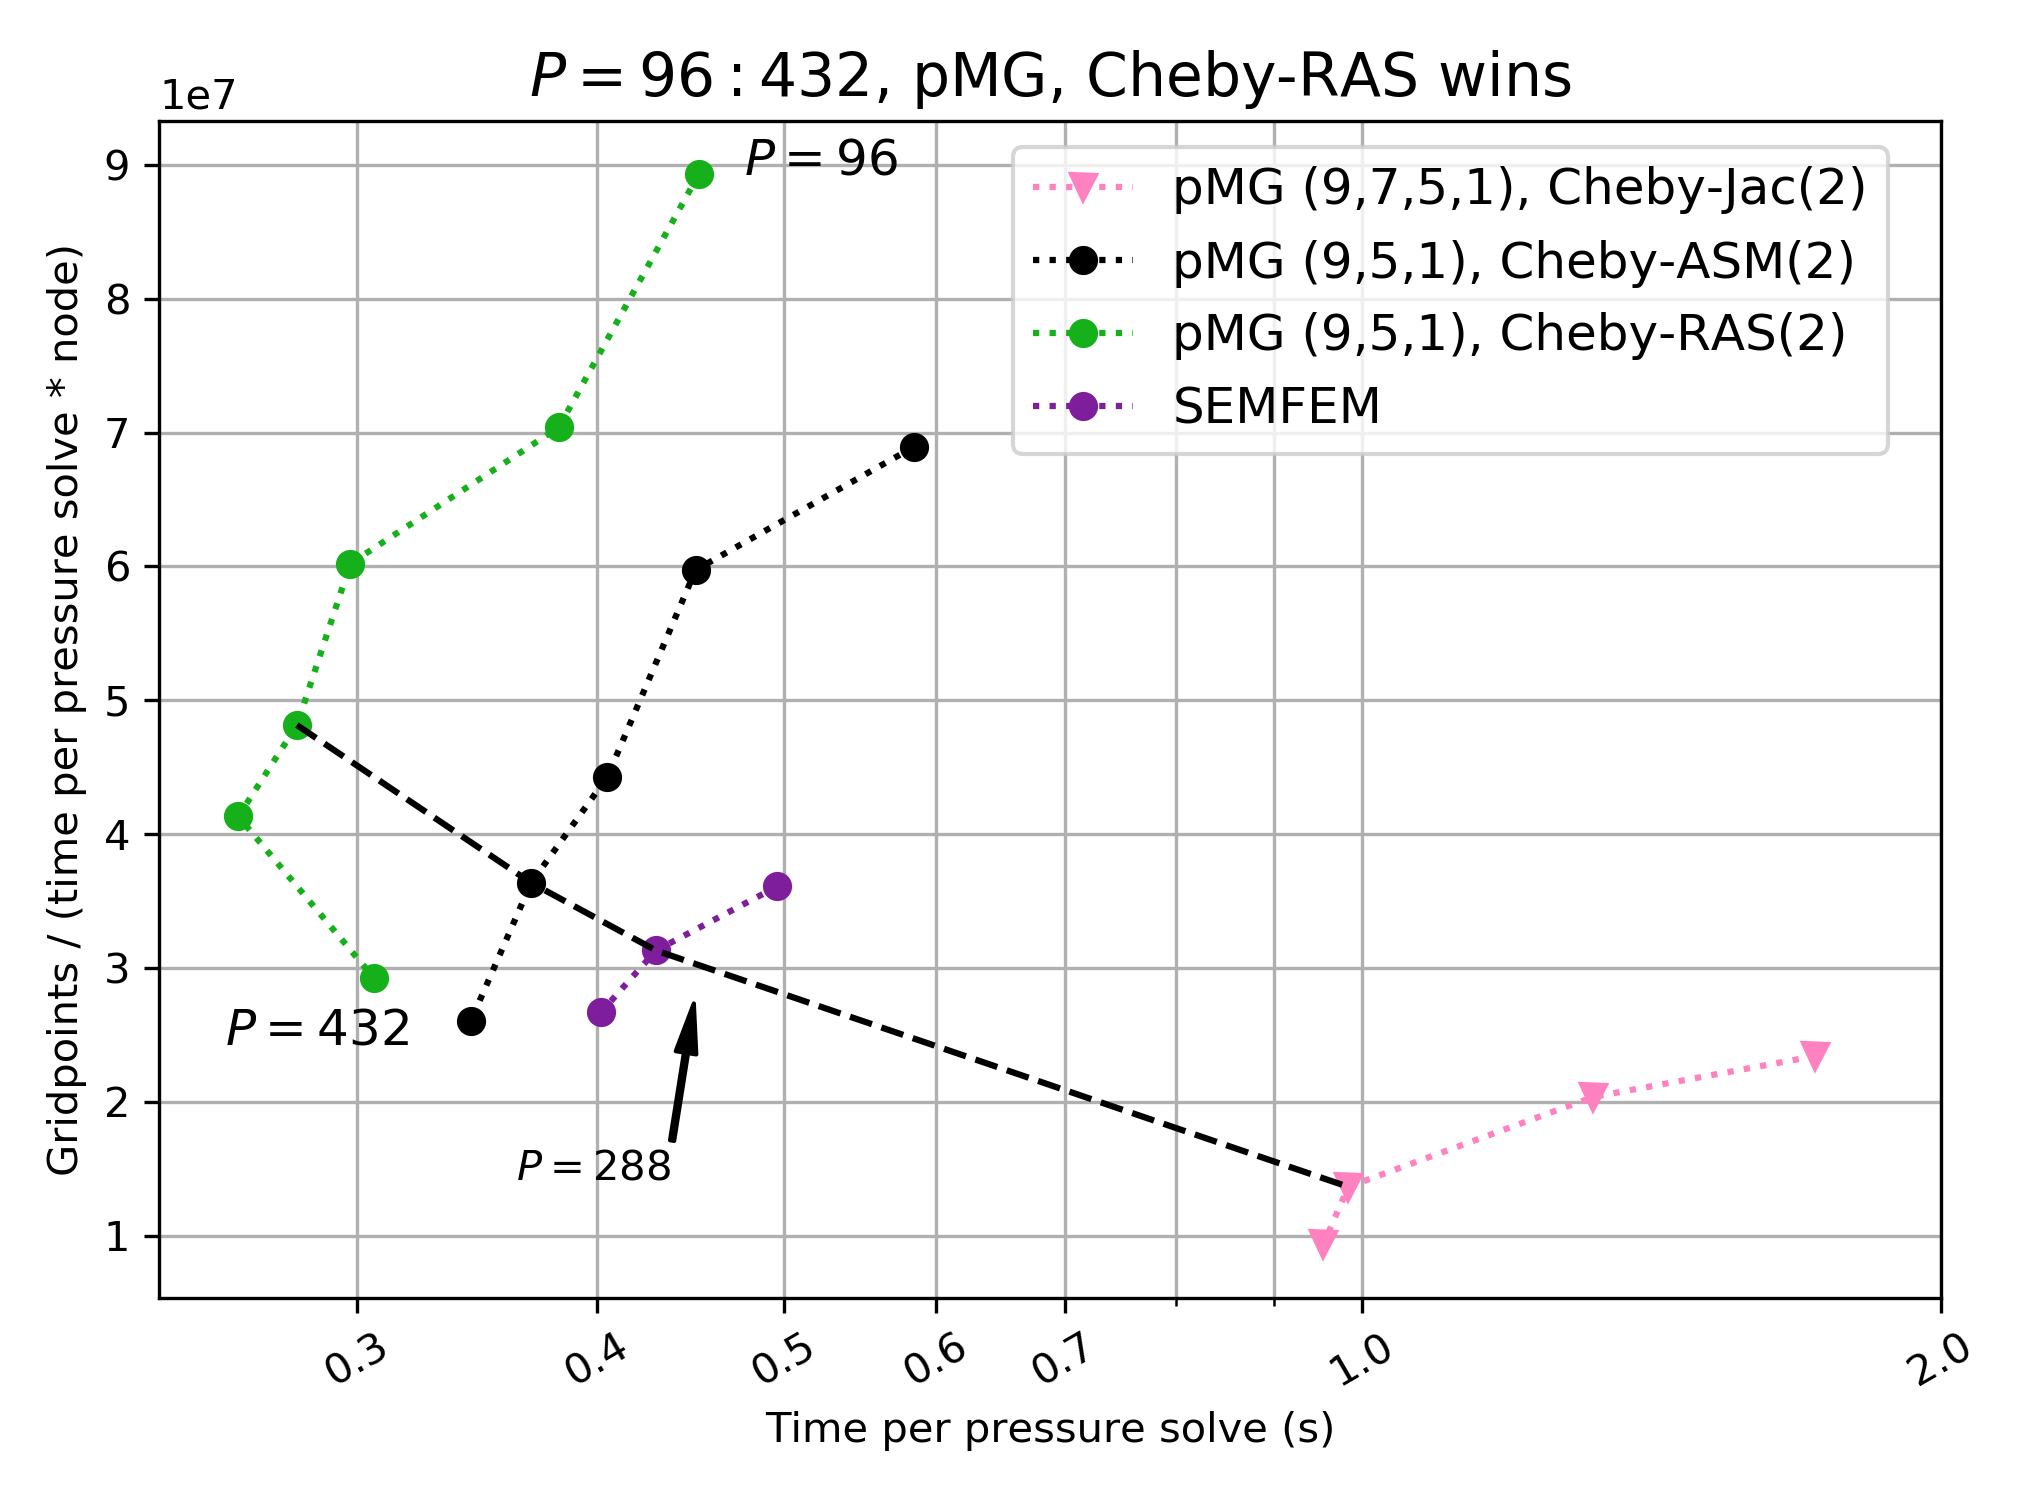
\includegraphics[width=\textwidth]{../figs/bsb-scaling.png}}
        \put(0.6,0.35){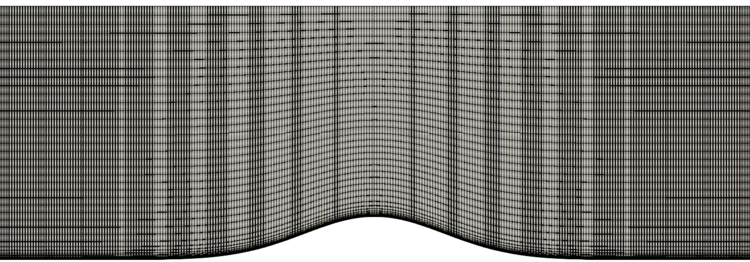
\includegraphics[width=0.3\textwidth]{../figs/BoeingSpeedBump.png}}
      \end{picture}}
    \captionsetup{labelformat=empty}
    \caption{
      \small
      Strong scaling results on Summit for the Boeing speed bump problem.
    }
  \end{figure}
\end{frame}
\begin{frame}
  %\begin{figure}
  %  \centering
  %  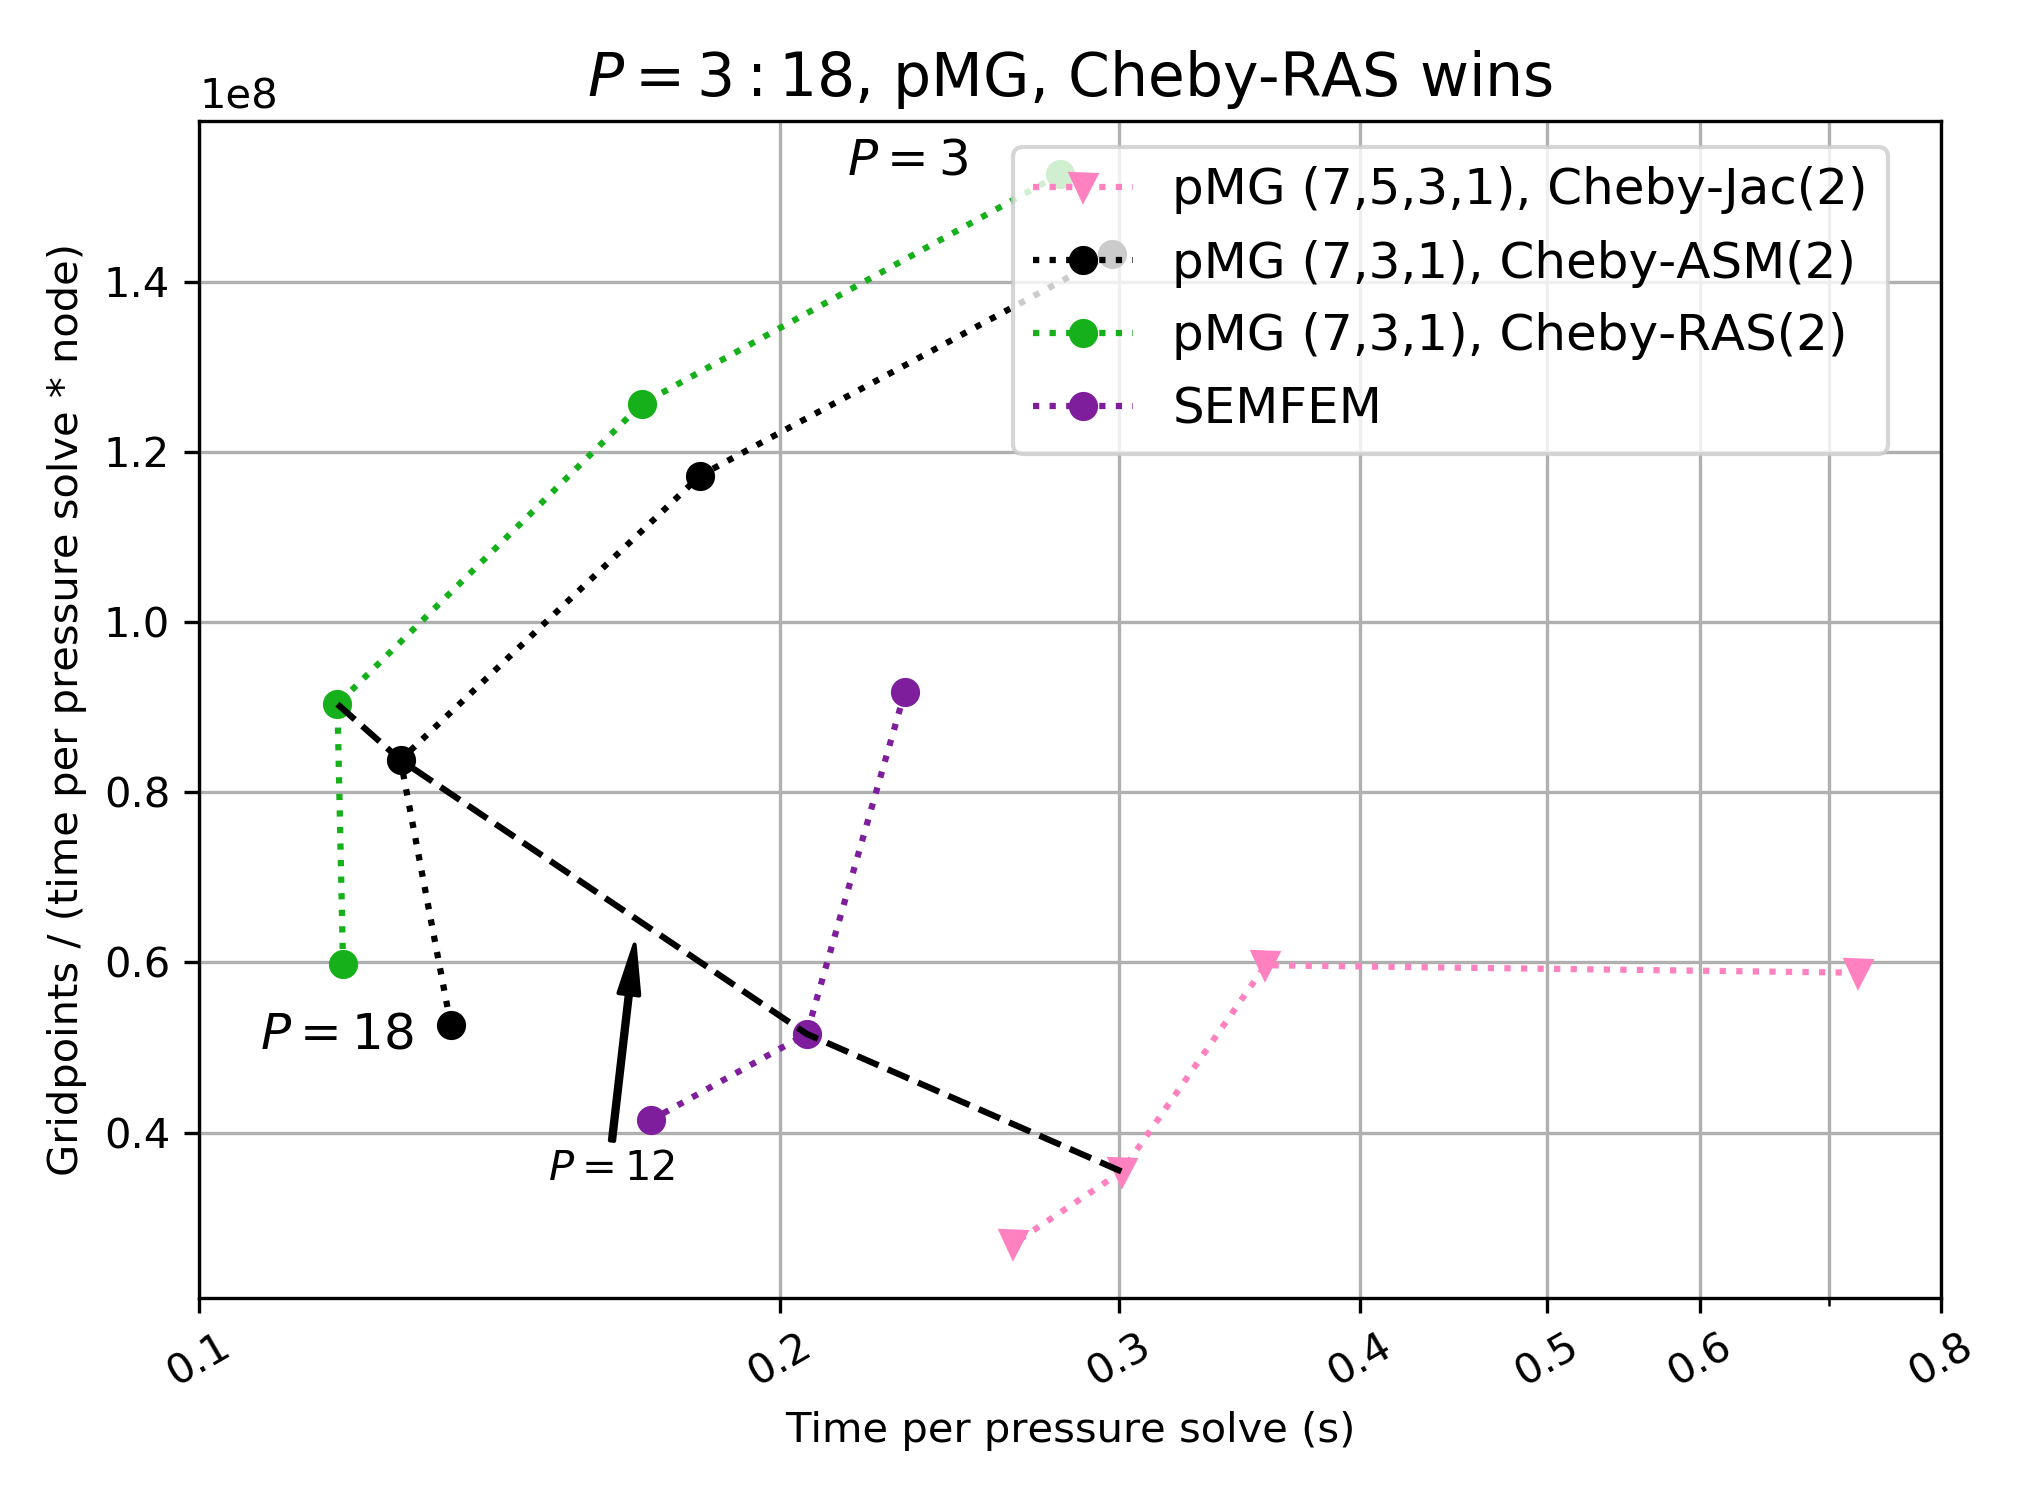
\includegraphics[width=\textwidth]{../figs/pb146-scaling.png}
  
  %  \vspace{-0.35cm}
  %  \captionsetup{labelformat=empty}
  %  \caption{
  %    \small
  %    Strong scaling results on Summit for the 146 pebble case.
  %  }
  %  \label{fig:pb146-scaling}
  
  %\end{figure}
  \begin{figure}
    {\setlength{\unitlength}{\textwidth}
      \begin{picture}(1,0.75)(0,0)
        \put(0.0,0.0){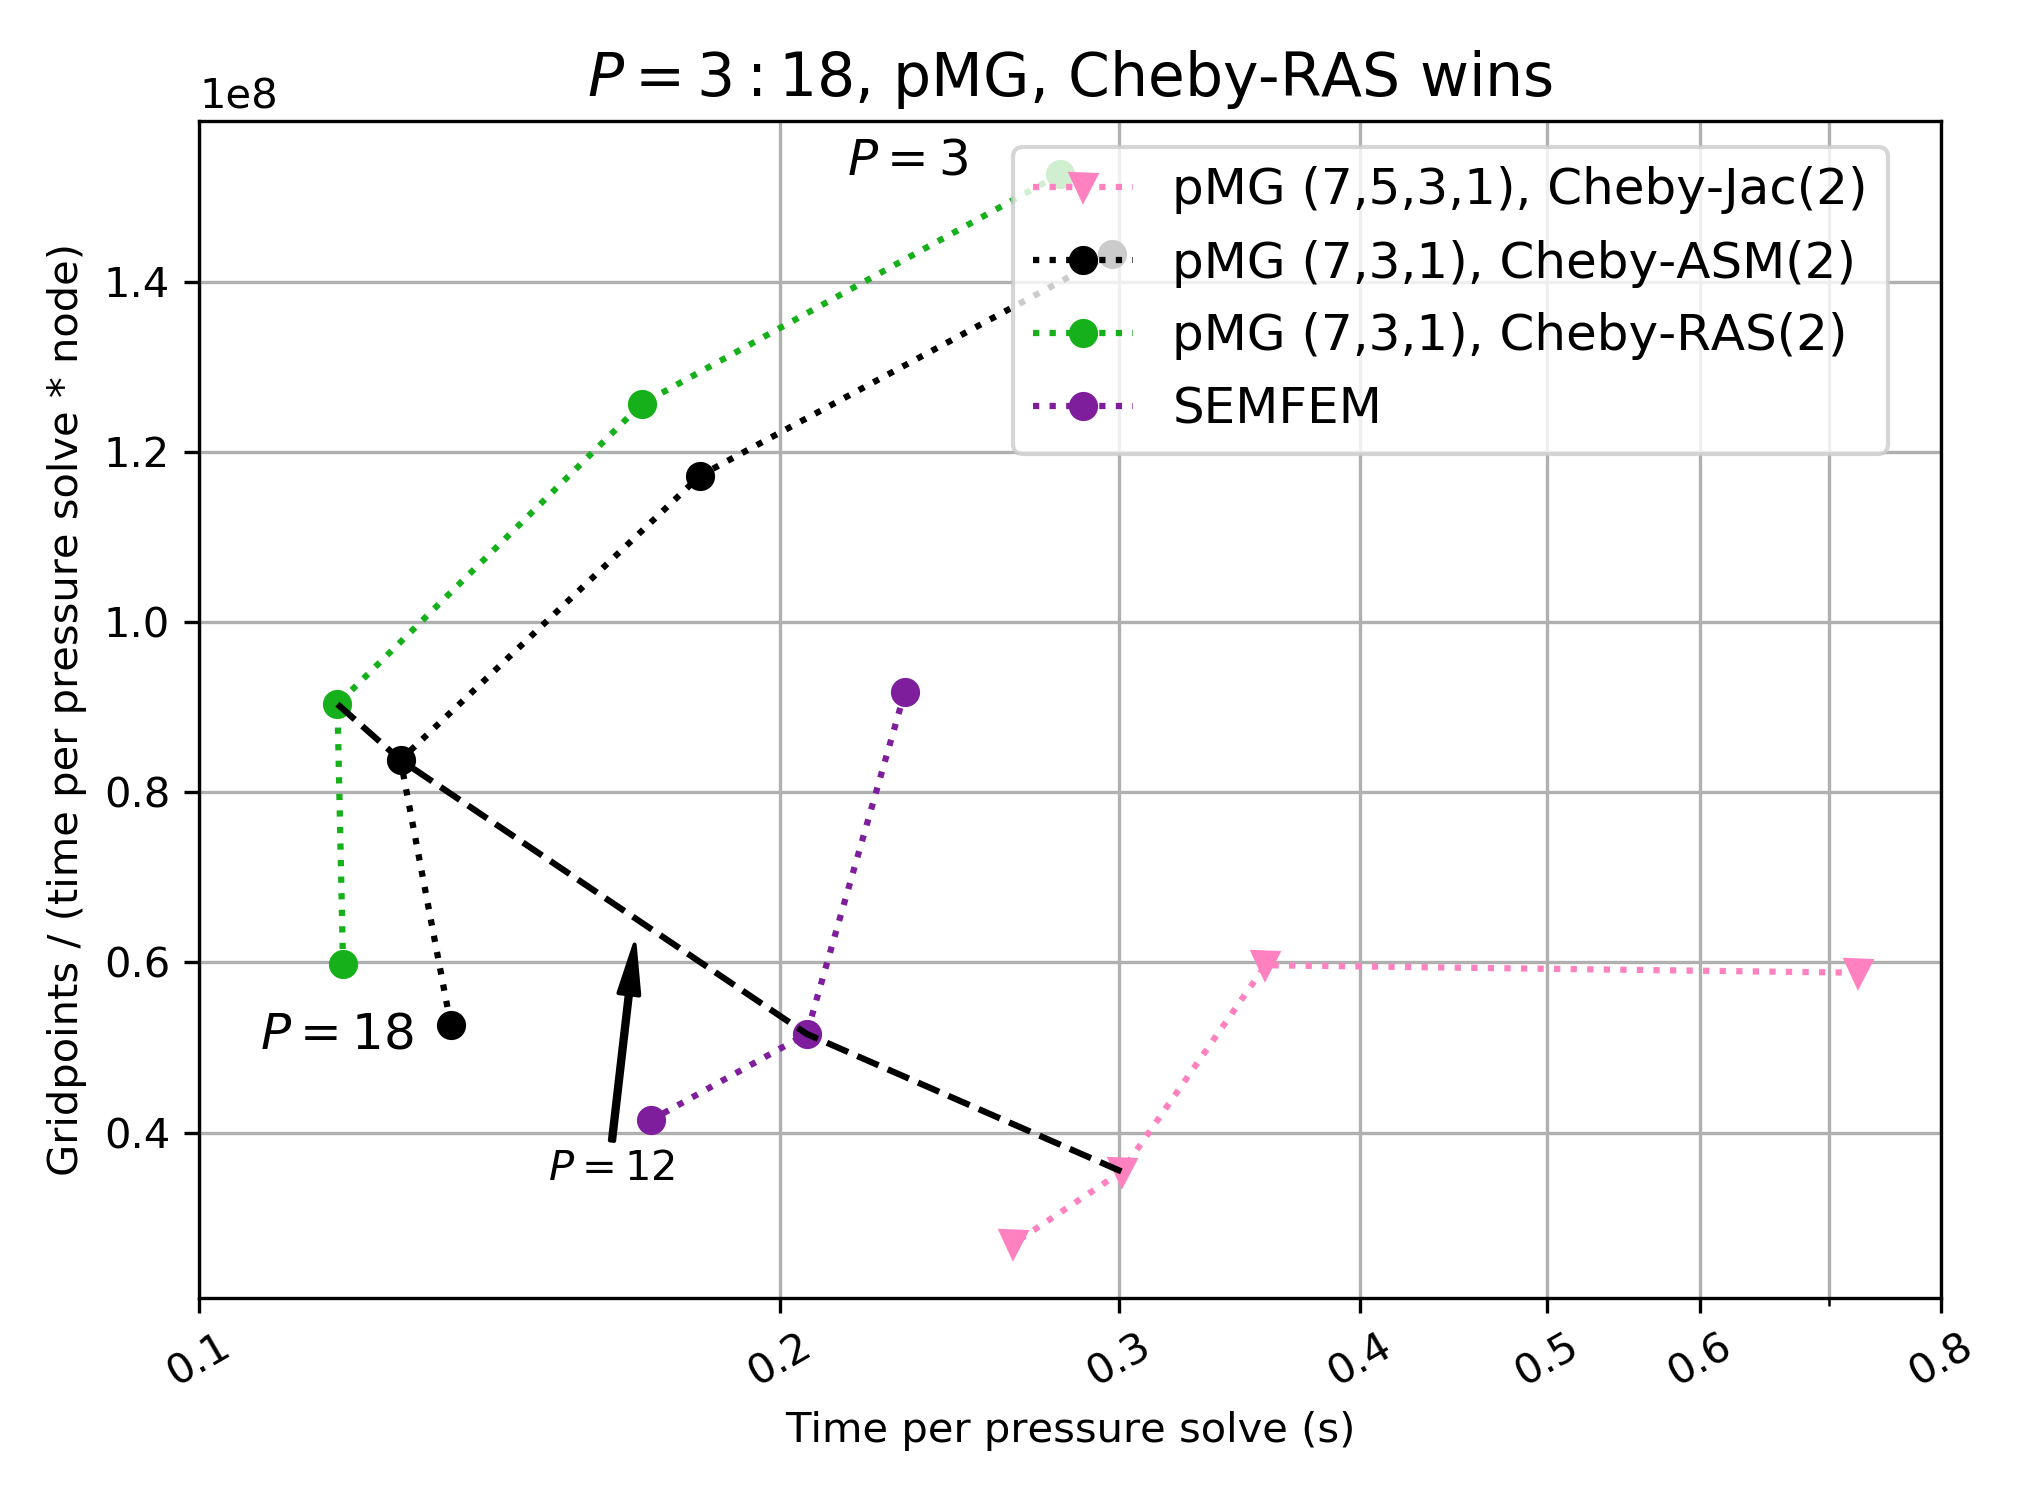
\includegraphics[width=\textwidth]{../figs/pb146-scaling.png}}
        \put(0.6,0.3){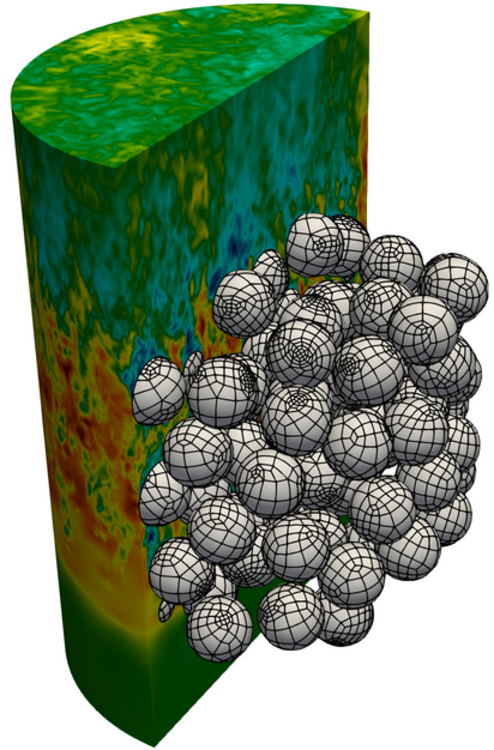
\includegraphics[width=0.15\textwidth]{../figs/pb146.png}}
      \end{picture}}
    \captionsetup{labelformat=empty}
    \caption{
      \small
      Strong scaling results on Summit for the 146 pebble case.
    }
  \end{figure}
\end{frame}

\begin{frame}
  %\begin{figure}
  %  \centering
  %  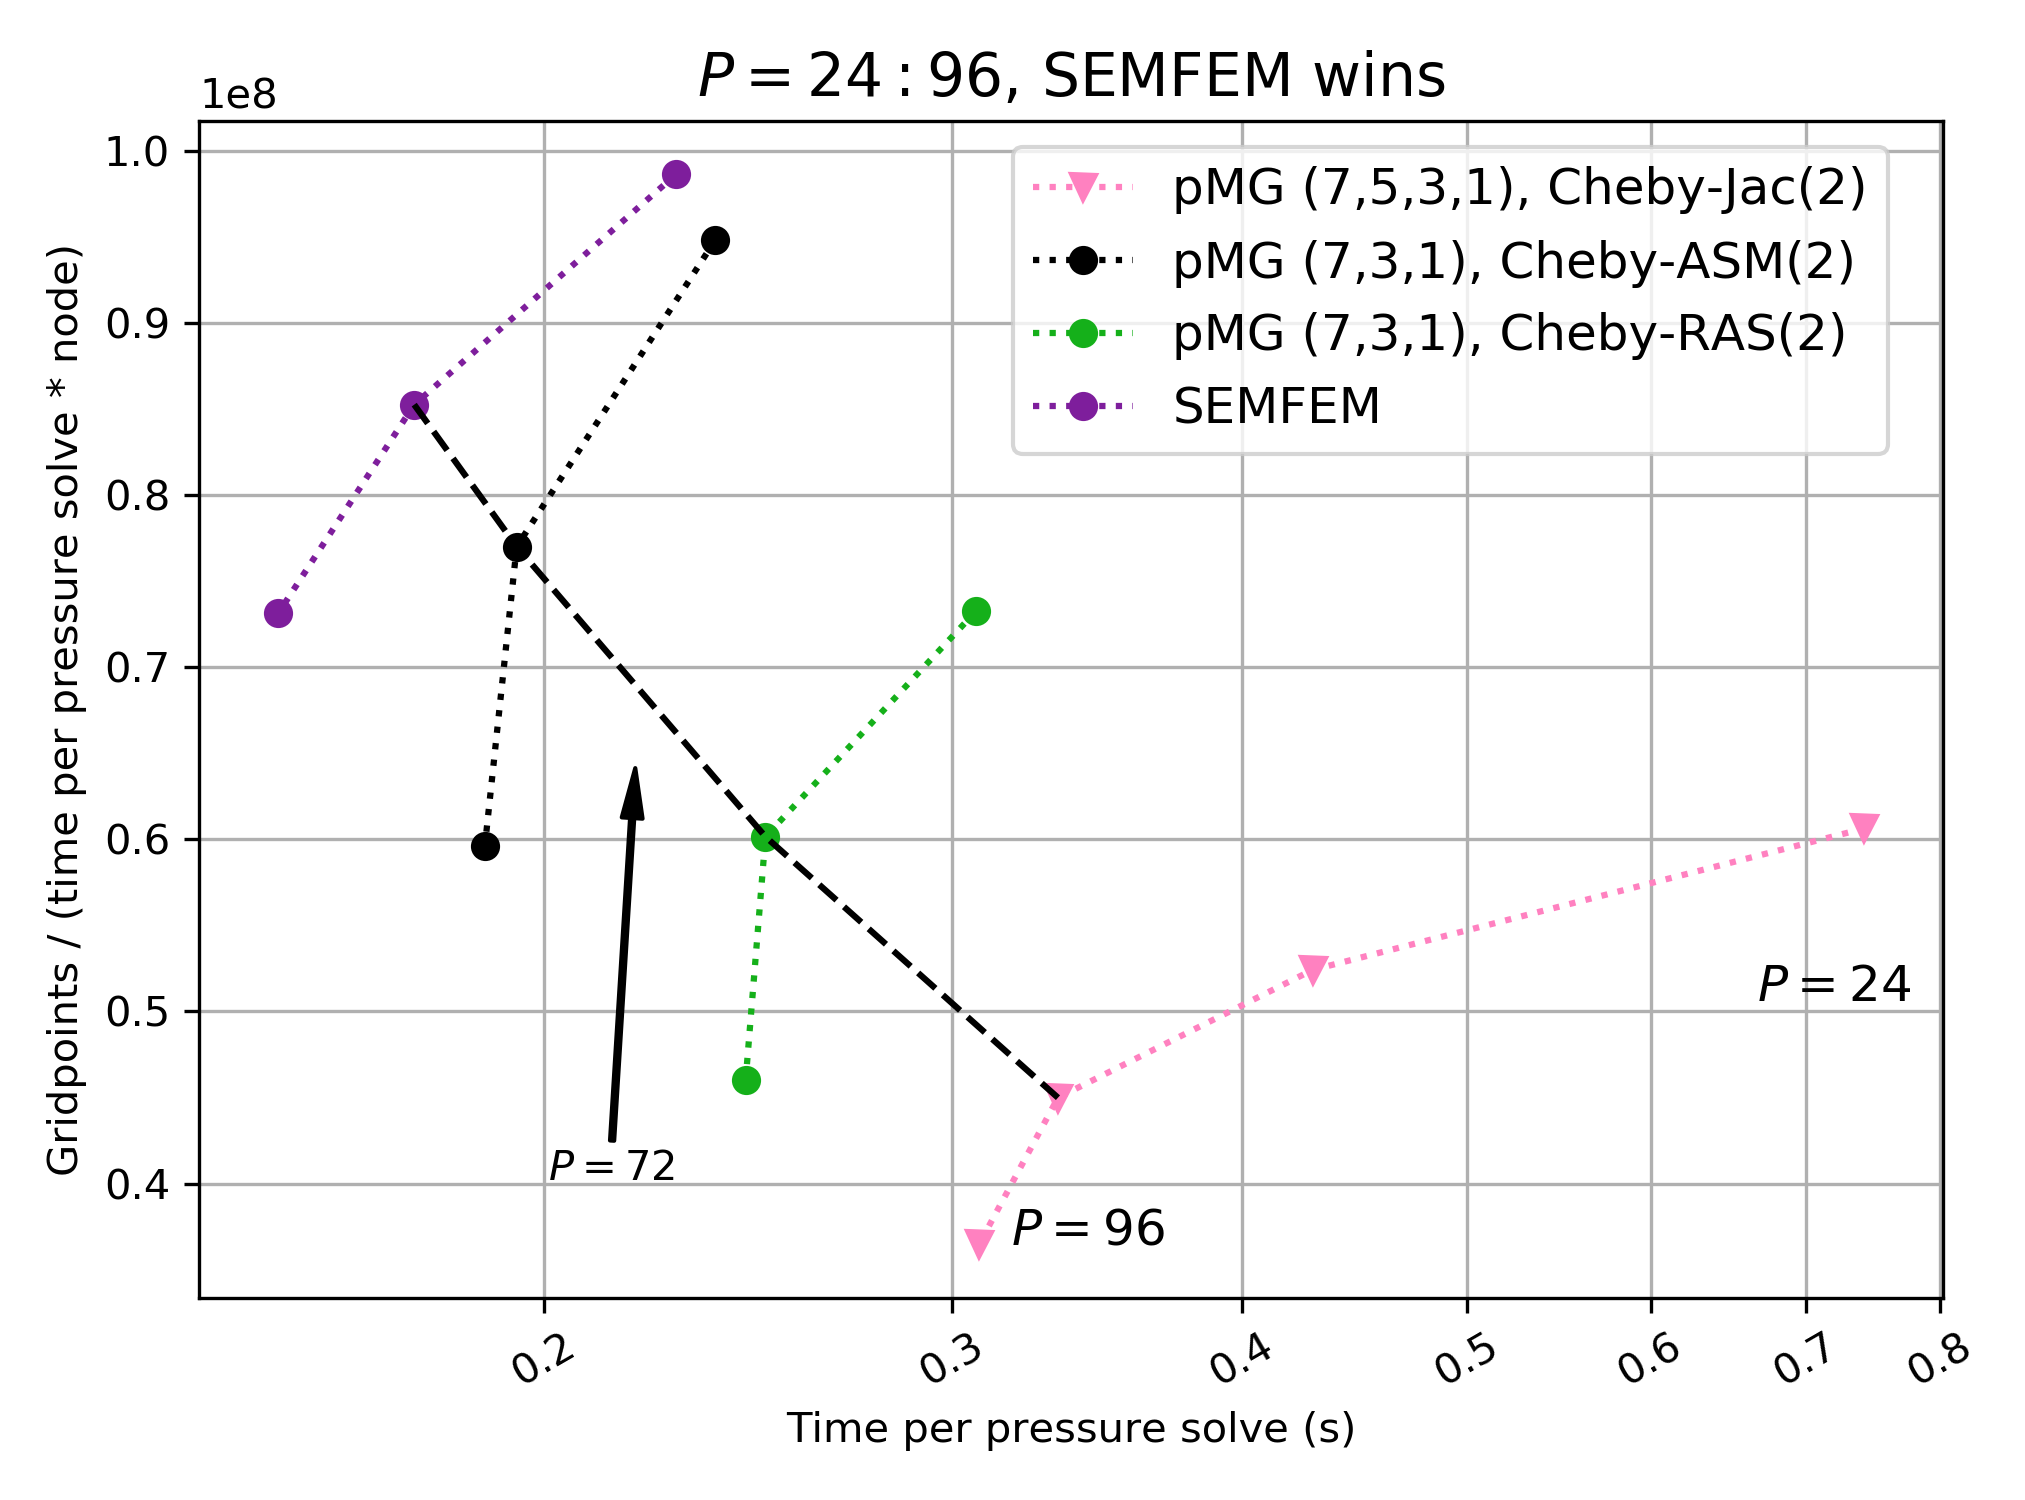
\includegraphics[width=\textwidth]{../figs/pb1568-scaling.png}
  
  %  \vspace{-0.35cm}
  %  \captionsetup{labelformat=empty}
  %  \caption{
  %    \small
  %    Strong scaling results on Summit for the 1568 pebble case.
  %  }
  %  \label{fig:pb1568-scaling}
  
  %\end{figure}
  \begin{figure}
    {\setlength{\unitlength}{\textwidth}
      \begin{picture}(1,0.75)(0,0)
        \put(0.0,0.0){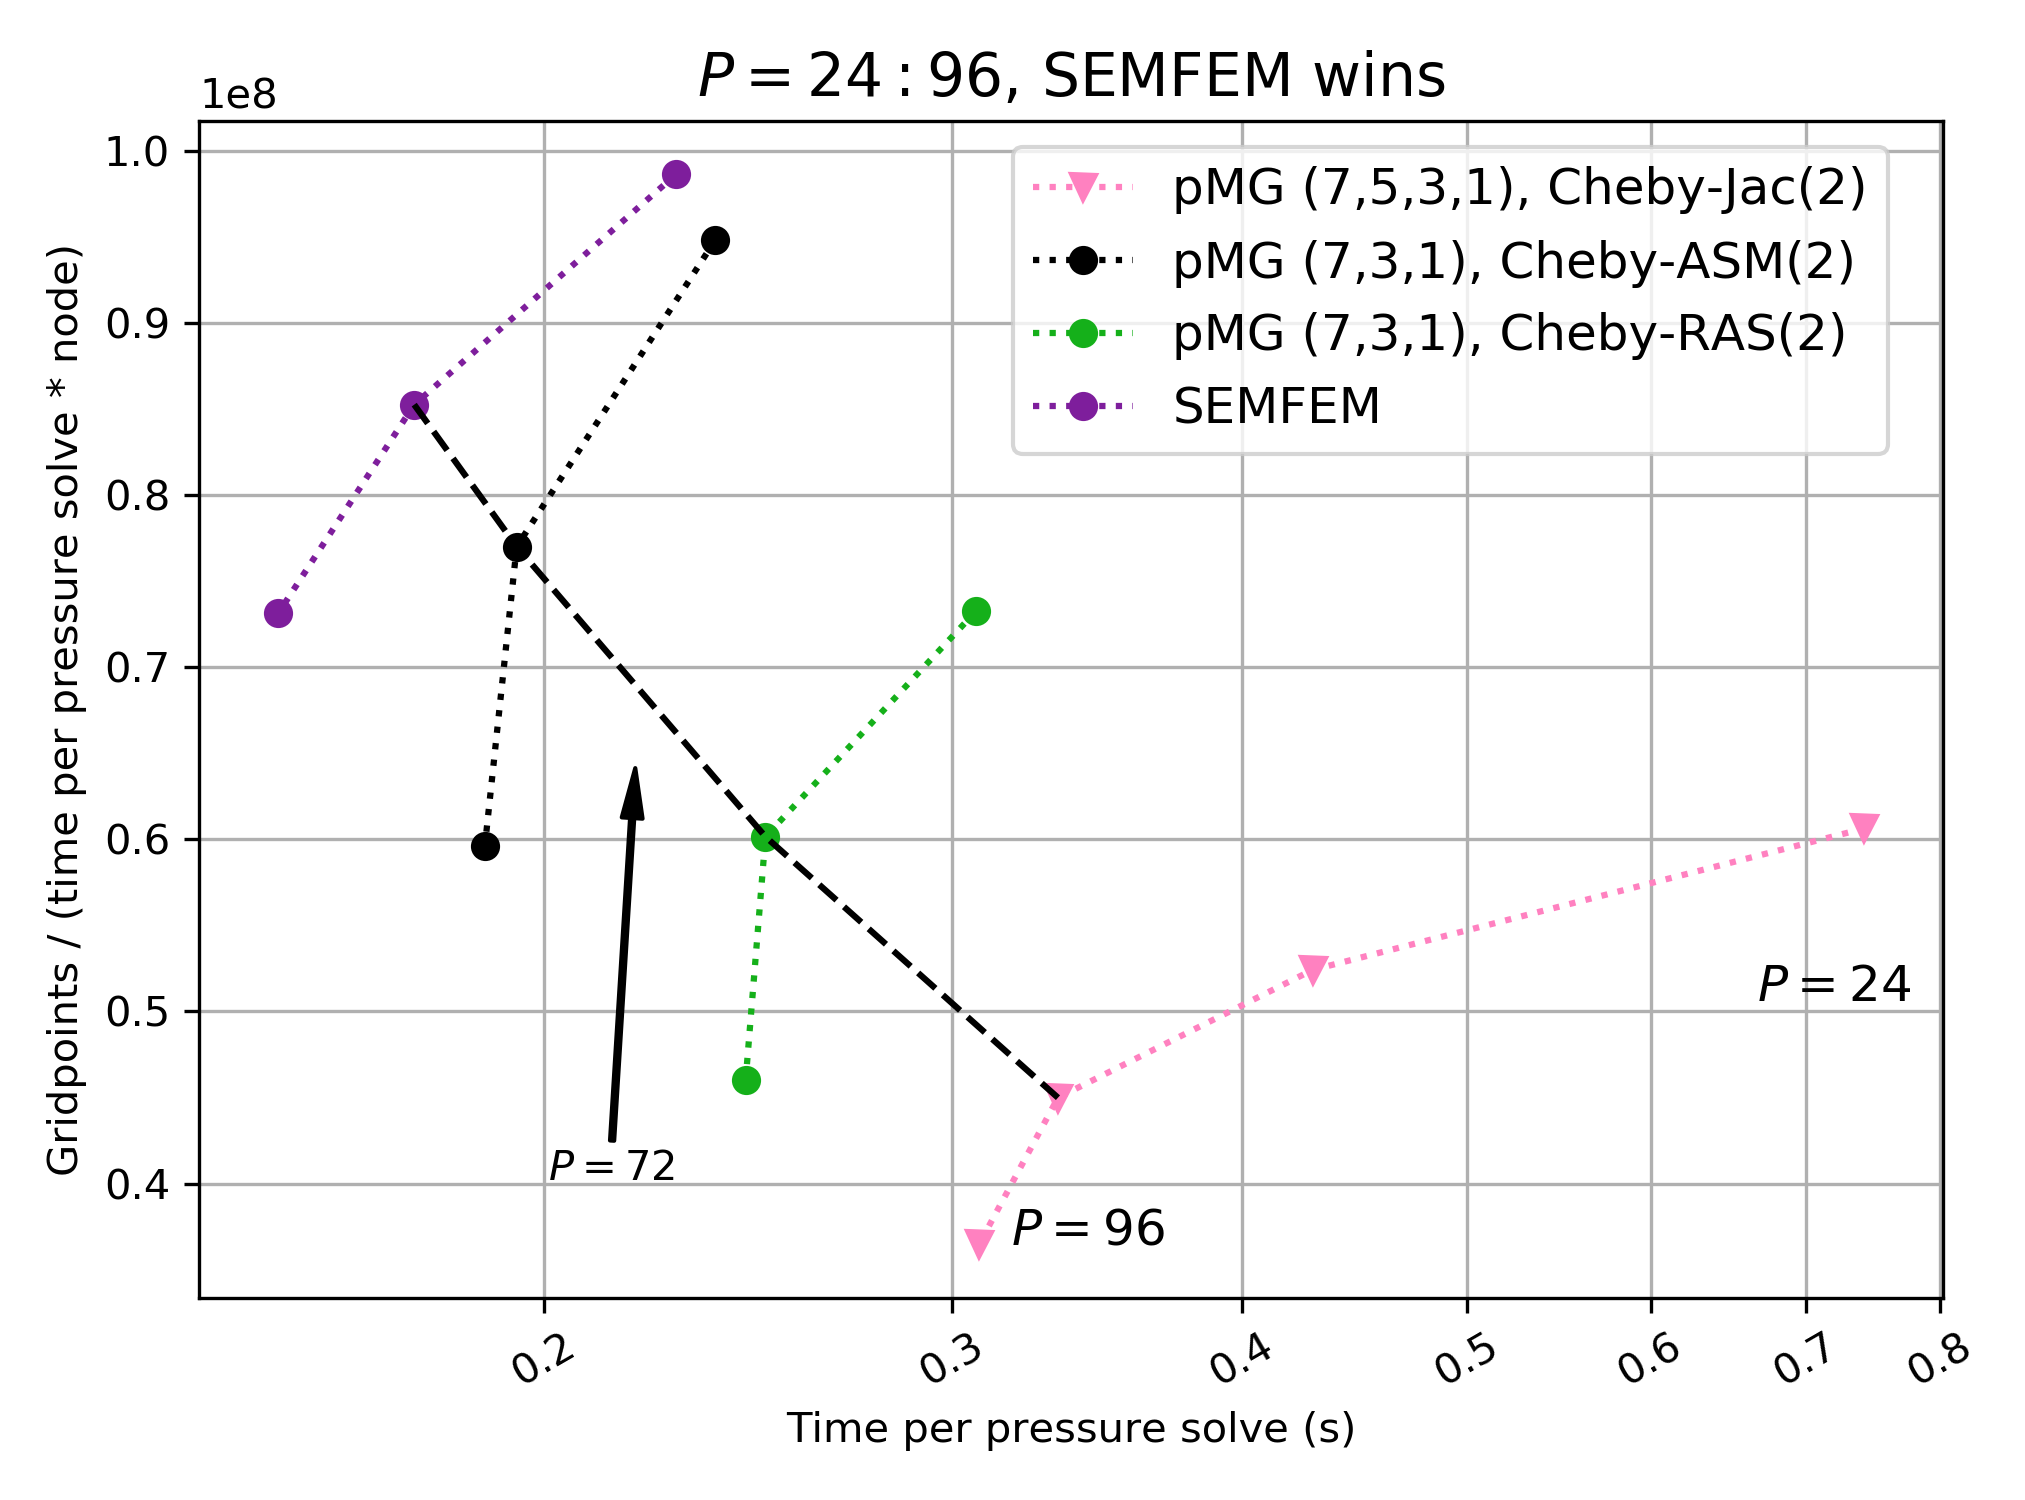
\includegraphics[width=\textwidth]{../figs/pb1568-scaling.png}}
        \put(0.6,0.3){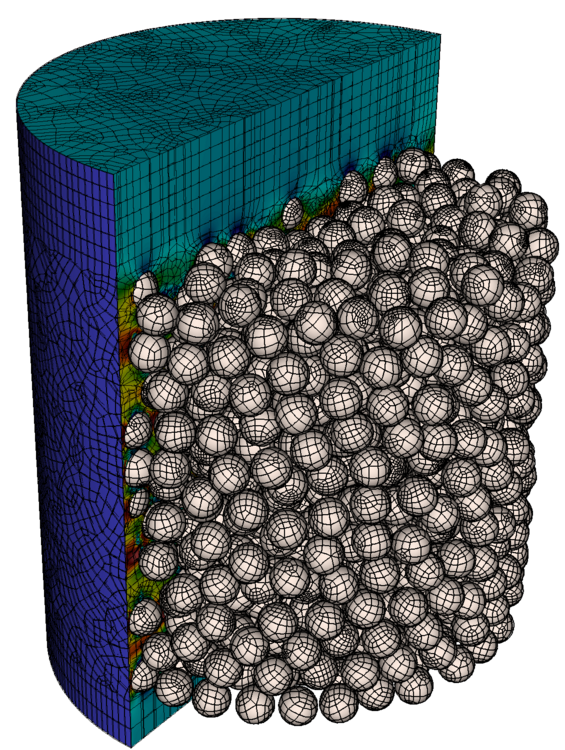
\includegraphics[width=0.15\textwidth]{../figs/pb1568.png}}
      \end{picture}}
    \captionsetup{labelformat=empty}
    \caption{
      \small
      Strong scaling results on Summit for the 1568 pebble case.
    }
  \end{figure}
\end{frame}

\begin{frame}
  %\begin{figure}
  %  \centering
  %  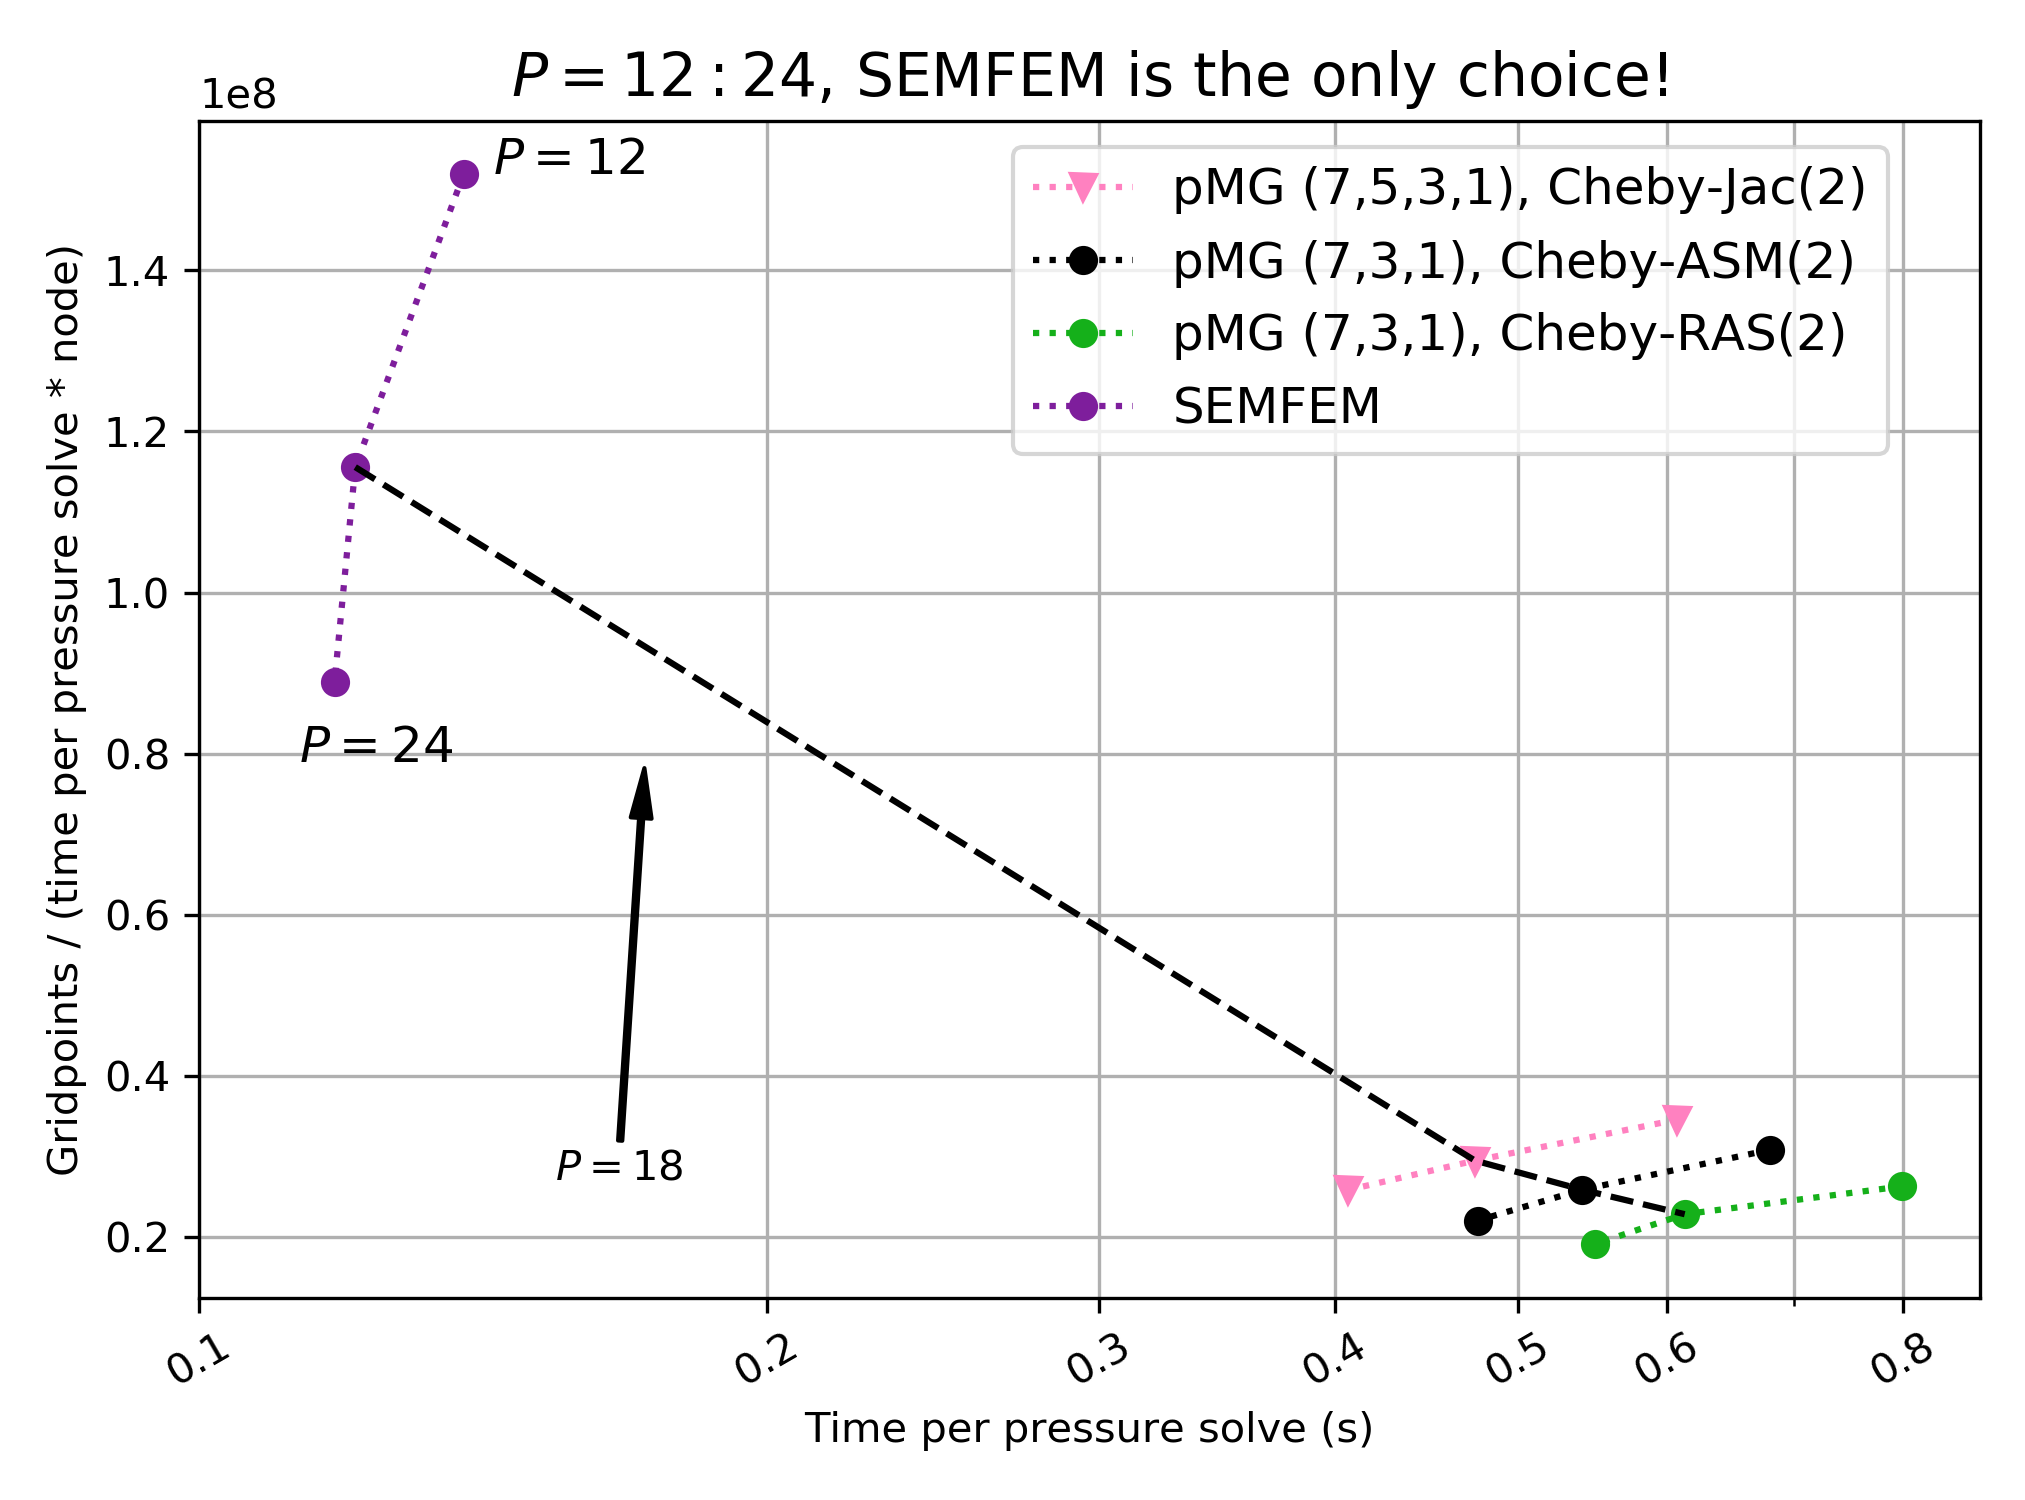
\includegraphics[width=\textwidth]{../figs/pb67-scaling.png}
  %  \vspace{-0.35cm}
  %  \captionsetup{labelformat=empty}
  %  \caption{
  %    \small
  %    Strong scaling results on Summit for the 67 pebble case.
  %  }
  %  \label{fig:pb67-scaling}
  %\end{figure}
  \begin{figure}
    {\setlength{\unitlength}{\textwidth}
      \begin{picture}(1,0.75)(0,0)
        \put(0.0,0.0){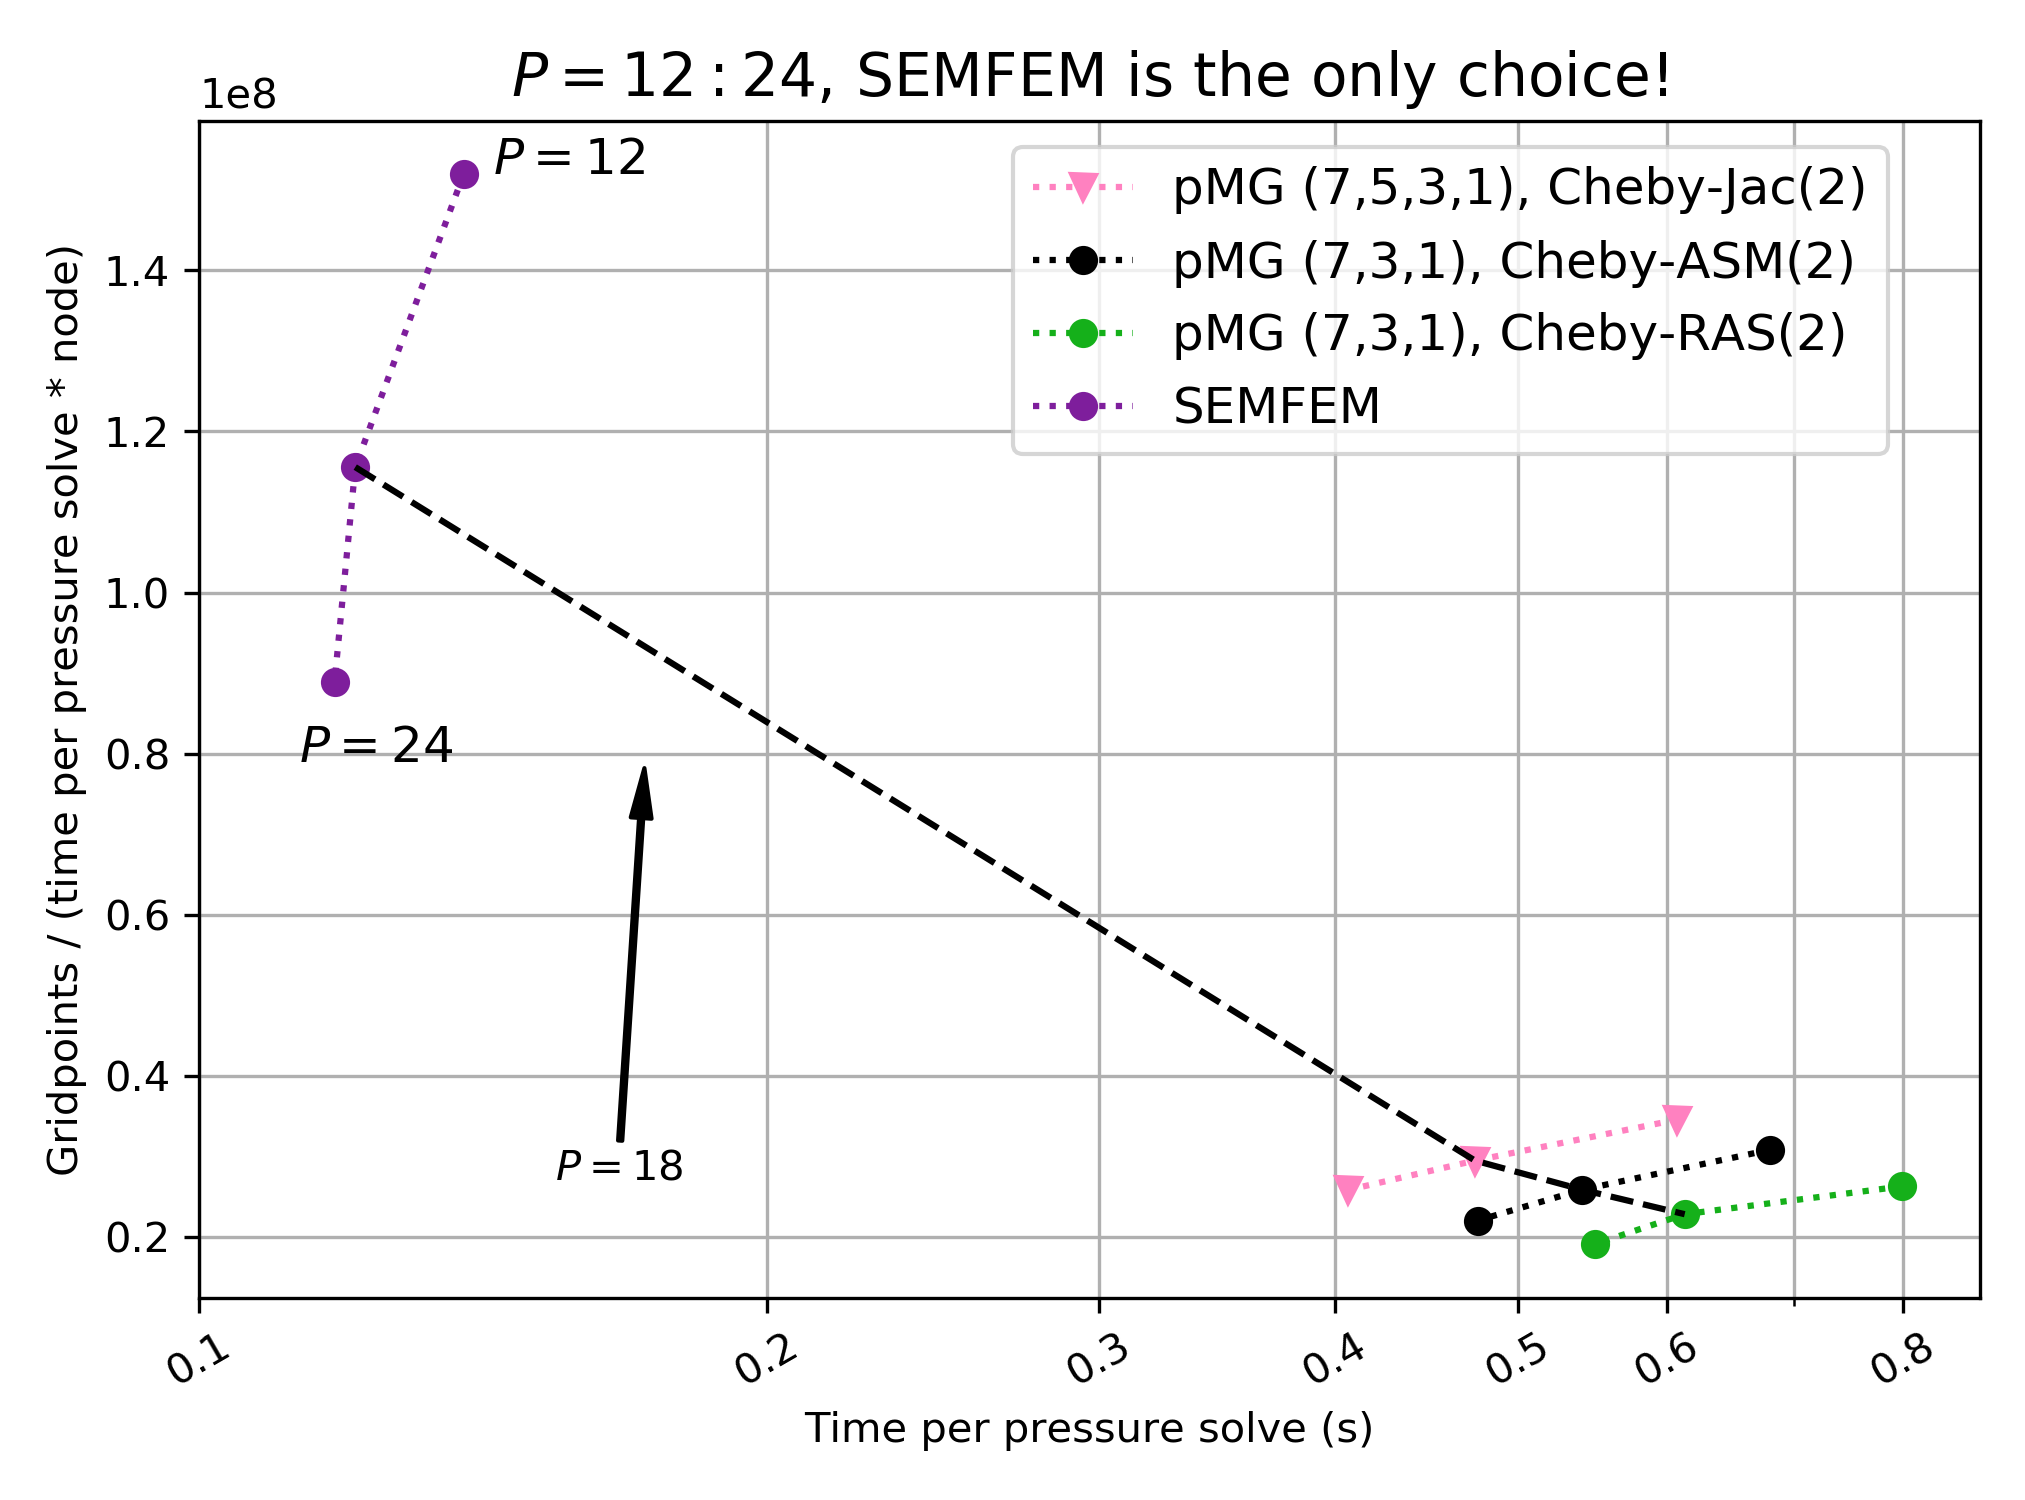
\includegraphics[width=\textwidth]{../figs/pb67-scaling.png}}
        %\put(0.65,0.525){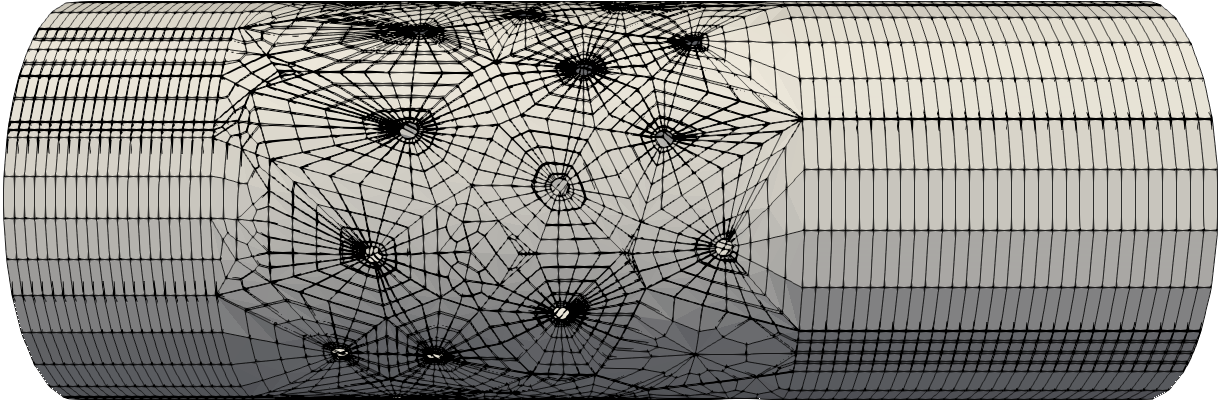
\includegraphics[width=0.3\textwidth]{../figs/peb67-side-profile.png}}
        %\put(0.7,0.3){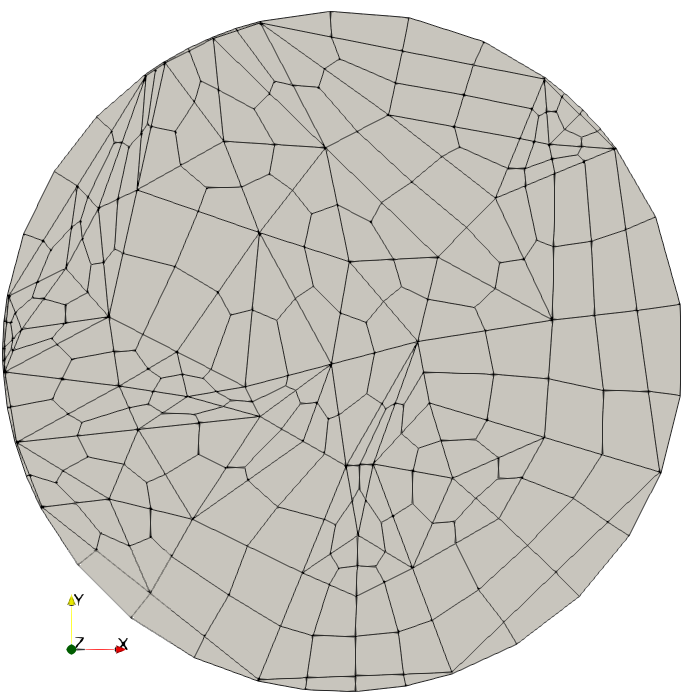
\includegraphics[width=0.2\textwidth]{../figs/peb67-face-profile.png}}
        \put(0.65,0.425){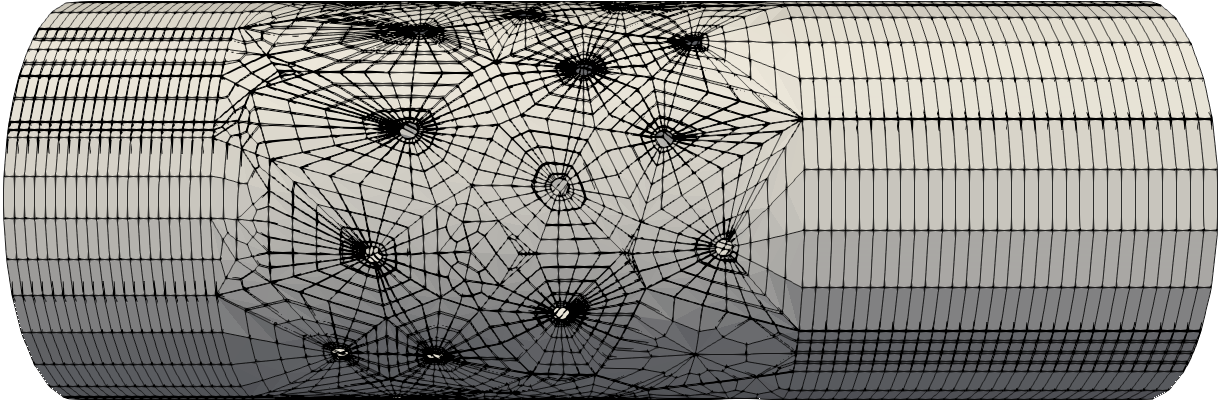
\includegraphics[width=0.3\textwidth]{../figs/peb67-side-profile.png}}
        \put(0.7,0.2){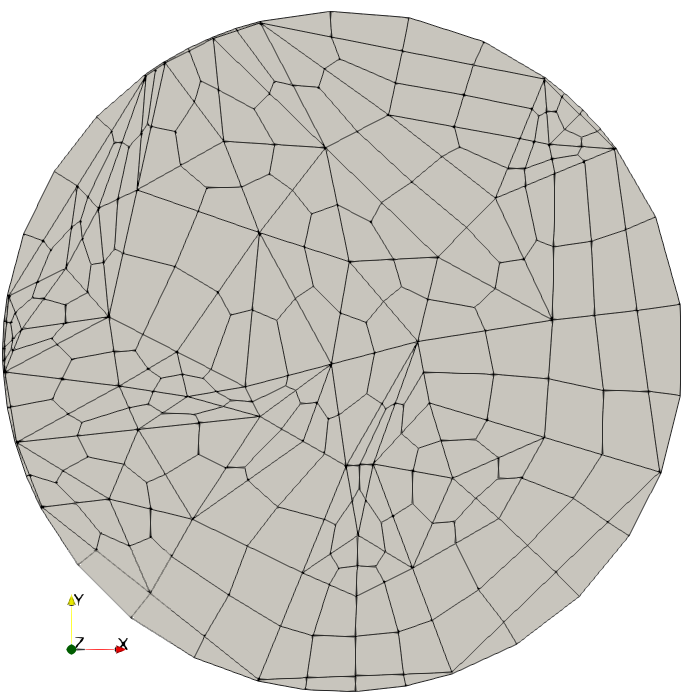
\includegraphics[width=0.2\textwidth]{../figs/peb67-face-profile.png}}
      \end{picture}}
    \captionsetup{labelformat=empty}
    \caption{
      \small
      Strong scaling results on Summit for the 67 pebble case.
    }
  \end{figure}
\end{frame}

%--------------------------------------------------------------------------
% Acknowledgements
%--------------------------------------------------------------------------
%\begin{frame}{Acknowledgements}
  \begin{itemize}
    \item This research is supported by the Exascale Computing Project (17-SC-20-SC),
          a collaborative effort of two U.S. Department of Energy organizations (Office of Science and the National Nuclear
          Security Administration) responsible for the planning and preparation of a capable exascale ecosystem,
          including software, applications, hardware,
          advanced system engineering and early testbed
          platforms, in support of the nation’s exascale computing imperative.
    \item Oak Ridge Leadership Computing Facility at Oak Ridge National
          Laboratory, Office of
          Science of the U.S. Department of Energy under
          Contract DE-AC05-00OR22725.
    \item Meshing/visualization provided by YuHsiang Lan, Ramesh Balakrishnan, David Alan Reger, and Haomin Yuan
    \item The reviewers of this work for their insightful comments and suggestions.
  \end{itemize}
\end{frame}

%--------------------------------------------------------------------------
% Citations
%--------------------------------------------------------------------------
%\begin{frame}[allowframebreaks]{References}
  %\setbeamerfont{bibliography item}{size=\footnotesize}
  %\setbeamerfont{bibliography entry author}{size=\footnotesize}
  %\setbeamerfont{bibliography entry title}{size=\footnotesize}
  %\setbeamerfont{bibliography entry location}{size=\footnotesize}
  %\setbeamerfont{bibliography entry note}{size=\footnotesize}
  %\bibliographystyle{apalike}
  %{\footnotesize
  %\bibliography{paper}
  %}
  \printbibliography
\end{frame}


\end{document}
